\chapter{Finite Element Analysis of IFB-HSB Hybrid Connection}
\label{ch5}

%%%%%%%%%%%%%%%%%%%%%%%%%%%%%%%%%%%%%%%
% IMPORTANT
\begin{spacing}{1.25} %THESE FOUR
\minitoc % LINES MUST APPEAR IN
\end{spacing} % EVERY
\onehalfspacing % CHAPTER
% COPY THEM IN ANY NEW CHAPTER
%%%%%%%%%%%%%%%%%%%%%%%%%%%%%%%%%%%%%%%

\section{Introduction}

As a joint length increases, problems arise when using  long or large bolted joints. First, owing to the presence of secondary members in the vicinity of the joint (e.g., stiffener and diaphragm), excessively long joints can interfere with secondary members. Therefore, it is necessary to shorten the length of the joint while maintaining design strength. Typically, a slip-critical joint combined with a weld is used to satisfy the design strength requirements of a joint. Previous studies have demonstrated that slip-critical bolted joints combined with welds are reliable and feasible \cite{solodov2021,Thomas2000,Chang2019361,KHANDEL2022107036}. Combinations of welded--bolted connections are widely used in steel structures. However, some environments, such as those offering insufficient space or requiring work at height, are not conducive to welding during onsite bridge construction. Welding also destroys the original coating of steel parts, which necessitates repainting the joints. As a result, the construction of combined welded--bolted connections is very difficult for steel bridge joints that require onsite joining. Appropriate methods are required to shorten the bolted joint without reducing its strength. \par

Second, as the length of the joint (defined as the spacing between the first and last fasteners in a joint) increases, the resistance that can bolt provide decreases to a value lower than the slip strength because the distribution of the bolts inside the joint becomes uneven. As the joint length increases with an increasing number of bolts in a line, the differential deformations in the main plate causes shear failure at the end bolts before all bolts can develop their full shearing strength. This ``unbuttoning'' phenomenon has been observed for all types of fasteners including rivets \cite{fisher1965behavior}. Bendigo et al.\cite{bendigo1963long} concluded that for longer connections, end bolts are sheared before all the bolts can develop their full shear strength. For short connections, the average shear stress is approximately 85\% that of a single bolt; however, for a 52.5 inch long connection, bolts only develop 60\% of their strength. Kamei et al. \cite{KAMEI2000} also showed that the serviceability limit strength decreases by approximately 2.5 $\%$ for each additional row.  Tan et al.\cite{Tan2022} considered that when the number of rows of bolts is more than 5, the force transmission ratio of the end bolt is 0.389.

Owing to the above issues, specifications for long-bolted joints, such as AASHTO , Eurocode, as well as Japanese and Chinese, all provide a reduction factor based on the length of the bolted joint\cite{AASHTO2020,eccs1985,isohtb,eurocode3-21,douji2017}. Furthermore, owing to uneven load sharing, the bolts cannot simultaneously fracture, and the ultimate limit bearing capacity decreases \cite{Takai2021BoltUnbuttoning,Peng2013FeaDimensions,peng2010,longstainless2022}. 

In this chapter, we proposed a method to reduce the joint length and maintains or slightly improves the strength without the limitation placed on splice plate sizes due to the congestion of secondary members, by combined the Interference fit bolt in the slip-critical bolted joint. The Finite element analysis was conduct to investigated the mechanical behavior of hybrid joints. We focused on adjusting the number of Interference fit bolts and the length of the joint to propose an optimized arrangement for Interference fit bolt. Additionally, we evaluated and classified the load transfer mode of the hybrid joint and classified the serviceability limit state.


\section{Definition of slip and bearing critical for hybrid joint}

Worldwide, the standard load-bearing capacity test on slip-critical bolted joints considers a two-bolt-connected specimen, and the load applicable to a splice plate with a relative displacement between 0.15 and 0.20 mm is applied as the ultimate slip load. However, Xu et al.\cite{xu2011} proposed that the standard for more than five rows of bolt connections is not applicable.  Peng et al.\cite{Peng2013FeaDimensions} conducted a slip test using a 12-row bolted joint. For the design slip load, the end bolt at the plate experienced 0.45 mm total slip, with an elastic deformation at the middle bolt of 0.1 mm. When the total slip at the end bolts reached 0.2 mm, the middle bolts experienced only 0.02 mm slip. This suggests that, by adhering to Japan's general slip assessment method \cite{AIJ2012AIJStructures}, it is unfeasible to ascertain the ultimate slip load for long-bolted joints. Comparing the load-carrying capacity of long- and short-bolted joints using this standard is also unattainable as the 0.15--0.2 mm slip range is inappropriate for connections consisting of more than five rows. A slip of 0.15--0.20 mm is already experiencing full slip for short connections, whereas for bolts in the long connection, the majority are not completely in slip. \par

For hybrid-bolted joints, the relative displacement is somewhat constrained by the Interference fit bolt installed at the end, such that the bolt on the inside could share more tensile force when evaluating the 0.2 mm relative displacement at the end. However, because the end bolts transmit tensile forces to the steel plate through the bearing, and the forces on the end bolts are considered to share more than 30\% of the tensile force before the slip of long-bolted joints \cite{Zhanghuazhi2000,chinarailway2005}, it is necessary to confirm whether the resistance on the Interference fit bolt exceeds the designed load-bearing capacity of the bolt. 

In this study, we defined the \ac{Bearing critical} of the hybrid-bolted joint when the end bolts of the hybrid bolt joint reached the shear yield strength or the end-bolt holes reached the bearing/shear strength (that is, the end bolt must satisfy Eq.\ref{eq-FV}). And the \ac{Slip critical} when the relative displacement reaches 0.2 mm. The \ac{0.2 mm slip} strength was defined with reference to the Architectural Institute of Japan \cite{AIJ2012AIJStructures} which states that slip occurs when the relative displacement reaches 0.2 mm, where the relative displacement for the main and splice plates is measured to be 10 mm from the end of the main plate. 

\begin{equation}
    F_{v,Ed.ser.end} \leq min\{F_{v,Rd.ser}, F_{b,Rd.ser}\}
    \label{eq-FV}
\end{equation}

where $F_{v,ED.ser}$ denotes the design shear force of the end bolt for the serviceability limit state (SLS), $F_{v,Rd.ser}$ denotes the design shear resistance per bolt at the SLS, and $F_{v,Rd.ser}$ denotes the design bearing resistance per bolt at the SLS.

\begin{equation}
    F_{vT,ED.ser} \leq F_{sT,ED.ser}
\end{equation}
The slip coefficient ($\mu_{0.2}$) was calculated using Eq.\ref{eq-slipcof}.
\begin{equation}
    \mu_{0.2} = \frac{P_{0.2slip}}{n \cdot m \cdot N_d}
    \label{eq-slipcof}
\end{equation}

where $n$ denotes the number of bolts, $m$ denotes the number of slip planes, $N_d$ denotes the axial force of the bolt before loading, and $P_{0.2slip}$ denotes the load when the joint's relative displacement reaches 0.2 mm.


\section{Finite element (FE) analysis}

\begin{figure}[htbp]
    \centering
    \includegraphics[width=0.95\textwidth]{imgs/ch5/femodelsize.pdf}
    \caption{Dimensional drawing of R12B2 case}
    \label{fig-modelsize}
\end{figure}

\subsection{Modelling methodology}

A general-purpose structural analysis software, Abaqus / Standard 2020, was utilized to perform three-dimensional elastoplastic finite-displacement analysis \cite{Smith2020}. \par
The analytical model was based on a 12-row bolted friction joint (the joint length was 825 mm from the first-out to the inner end bolt), as shown in Fig. \ref{fig-modelsize}. The thickness of the main and splice plates was set to 75 mm and 38 mm, respectively. The load was applied by forced displacement at the end surface of the main plate, and the analysis was conducted for half of the model, with the center of the joint in the longitudinal direction set as the axis of symmetry. Referring to \cite{Shimozato2008ExperrimentalModel}, the Interference fit bolt did not completely simulate the knurling part; instead, it achieved a bearing state before applying a tensile load by changing the diameter of the shaft. The diameter of the Interference fit bolt was set to the same as bolt hole (23.5 mm), and the diameter of the High-strength hexagon bolt for slip-critical connection (hereafter known as High-strength hexagon bolt) was set to 22 mm. \par

The material properties and nominal stress-- nominal strain curves of the materials used in the analysis are listed in Tables \ref{tab-mateproper} and \ref{fig-matpro}. The SM490Y material was used for the main and splice plates  \cite{JISsteel}, and both the friction- and bearing-type--high-strength bolts  (HSB) had F10T material properties \cite{JISbolt}, which is equivalent to ASTM A490 or Grade 10.9 \cite{ASTM-bolt,ISO-bolt}. All the material properties were modeled using a trilinear model with a quadratic gradient of $E/100$, and the ultimate strength was considered. \par

The mesh division and selection of elements were obtained from a study by Ju. S. H. et al. \cite{ju2004-boltfea}. Figure  \ref{fig-femesh} illustrates the mesh division of the analytical model. The approximate global size of the elements in the FE models was 20 mm, and the total number of elements in the FE models was 251,487. The mesh size of the main plate was set to 1/15 (5 mm) relative to the plate thickness direction. The mesh size of the High-strength hexagon bolt was set to 2 mm, the Interference-body bolt to 2.9 mm, washer to 3 mm, and nut to 5 mm. The elements applied in the model were three-dimensional--eight-node solid elements with a reduced integration (C3D8R). \par
Contact boundary conditions were set between the main and splice plates, bolt-hole wall and bolt shank, and washer and splice plates to reproduce the conditions of contact, separation, and fixation, as shown in Fig. \ref{fig-contactp}. The surface-to-surface discretization method was employed to prevent surface penetration, whereas the finite sliding tracking approach was utilized to enable the unrestricted movement of the contact surfaces. For boundary nonlinearity, hard contact and penalty friction were employed to define the normal and tangential behaviors of the contact pairs, and the friction was modeled using isotropic Coulomb friction. 

According to the Japan Road Association(JRA) -- Specifications for Highway Bridges, the minimum slip coefficient is specified as 0.40 for faying surfaces without coatings (excluding mill scale), and 0.45 for surfaces coated with inorganic zinc coatings \cite{douji2017,shishin2009}. In this study, a spcified minimum value of 0.4 was chosen as the friction coefficient. \par
To model the bolts, we referred to a previous study \cite{Kim2007,hung1996,Shimozato2008ExperrimentalModel}. In the first step of the analysis, the bolt was tightened using the Abaqus option bolt load and design bolt preload (205 kN), and the bolt was fixed at its current bolt-shank length in the subsequent steps. This method allows the bolt length to remain unchanged, such that the force in the bolt can change according to the response of the model \cite{Smith2020}. In the second step, forced displacement was applied to the end of the main plate.


\begin{table}[htbp]
\caption{Material properties}
\label{tab-mateproper}
\scalebox{0.8}{
\begin{tabular}{@{}cccccc@{}}
\toprule
\textbf{Member} &
  \textbf{Material} &
  \textbf{\begin{tabular}[c]{@{}c@{}}Young's modulus\\ {[}$N/mm^2${]}\end{tabular}} &
  \textbf{\begin{tabular}[c]{@{}c@{}}Poisson's ratio\\$v$ \end{tabular}} &
  \textbf{\begin{tabular}[c]{@{}c@{}}Yield strength\\ {[}$N/mm^2${]}\end{tabular}} &
  \textbf{\begin{tabular}[c]{@{}c@{}}Ultimate strength\\ {[}$N/mm^2${]}\end{tabular}} \\ \midrule
\begin{tabular}[c]{@{}c@{}}Main plate \\ Splice plate\end{tabular} &
 SM490Y &  \multirow{2}{*}{200,000} & \multirow{2}{*}{0.3} &  365 &  491 \\
High-strength bolt &  F10T / B10T & & &  900 &  1091 \\ \bottomrule
\end{tabular}}
\end{table}

\begin{figure}[htbp]
    \centering
    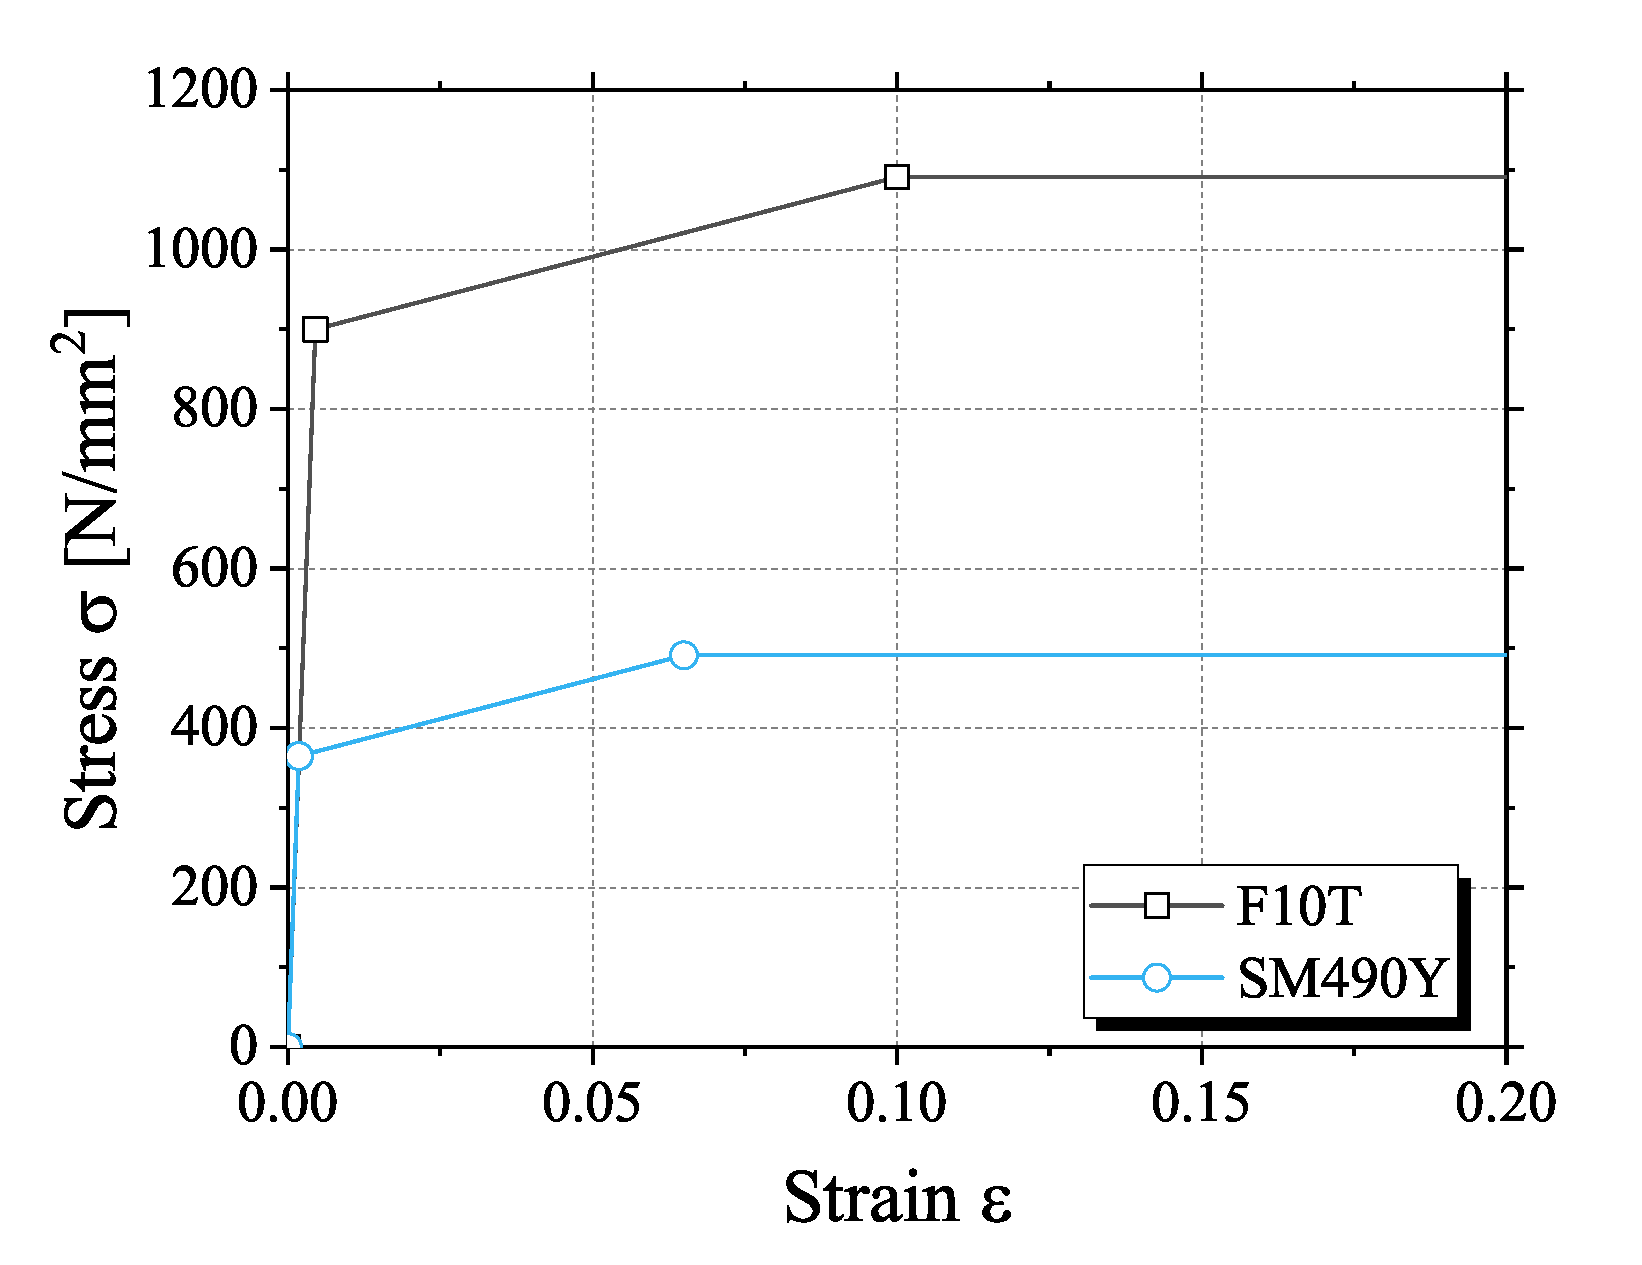
\includegraphics[width=0.5\linewidth]{imgs/ch5/mat-pro.eps}
    \caption{Nominal stress - Nominal strain curves of materials}
    \label{fig-matpro}
\end{figure}

\begin{figure}[htbp]
    \centering
    \includegraphics[width=0.95\textwidth]{imgs/ch5/femesh.pdf}
    \caption{FE model mesh division}
    \label{fig-femesh}
\end{figure}

\begin{figure}[htbp]
    \centering
    \includegraphics[width=0.5\linewidth]{imgs/ch5/contactp.pdf}
    \caption{Surface definition for contact pairs}
    \label{fig-contactp}
\end{figure}

\subsection{Validation of FE model}

The modeling methods of  the original R12-O case in this analysis refer to the modeling method used in previous research \cite{Peng2013FeaDimensions}, and the same analysis results were obtained.

We also referred to previously published experimental data \cite{peng2010} from other analyses to verify the modeling methods used in this study. The experimental setup is illustrated in Fig.\ref{fig-testset}, and the result of analysis and experiment is shown in Fig.\ref{fig-validloadrd}. The relative displacement taken from a distance of 10 mm from the inner end of the plate forms the reference for this experiment.

The analysis results were almost identical to the test results. Because the analysis used the penalty method to model contact and the static friction coefficient and isotropic Coulomb friction method to model friction, after the slip, the analysis would not be similar to the experiment in which the slip behavior was changed to kinetic friction and load reduction occurred. Therefore, the curve shape after the slip occurred, and the analysis and experimental results deviated. Therefore, the modeling methods used in this analysis can be considered valid.

For the hybrid joint, although the theoretically calculated value is the same as the analysis result, the verification of the mechanical behavior and failure mode of the hybrid joint will be conducted in a future study.

\begin{figure}[htbp]
    \centering
    \begin{subfigure}[t]{0.4\textwidth}
        \centering
        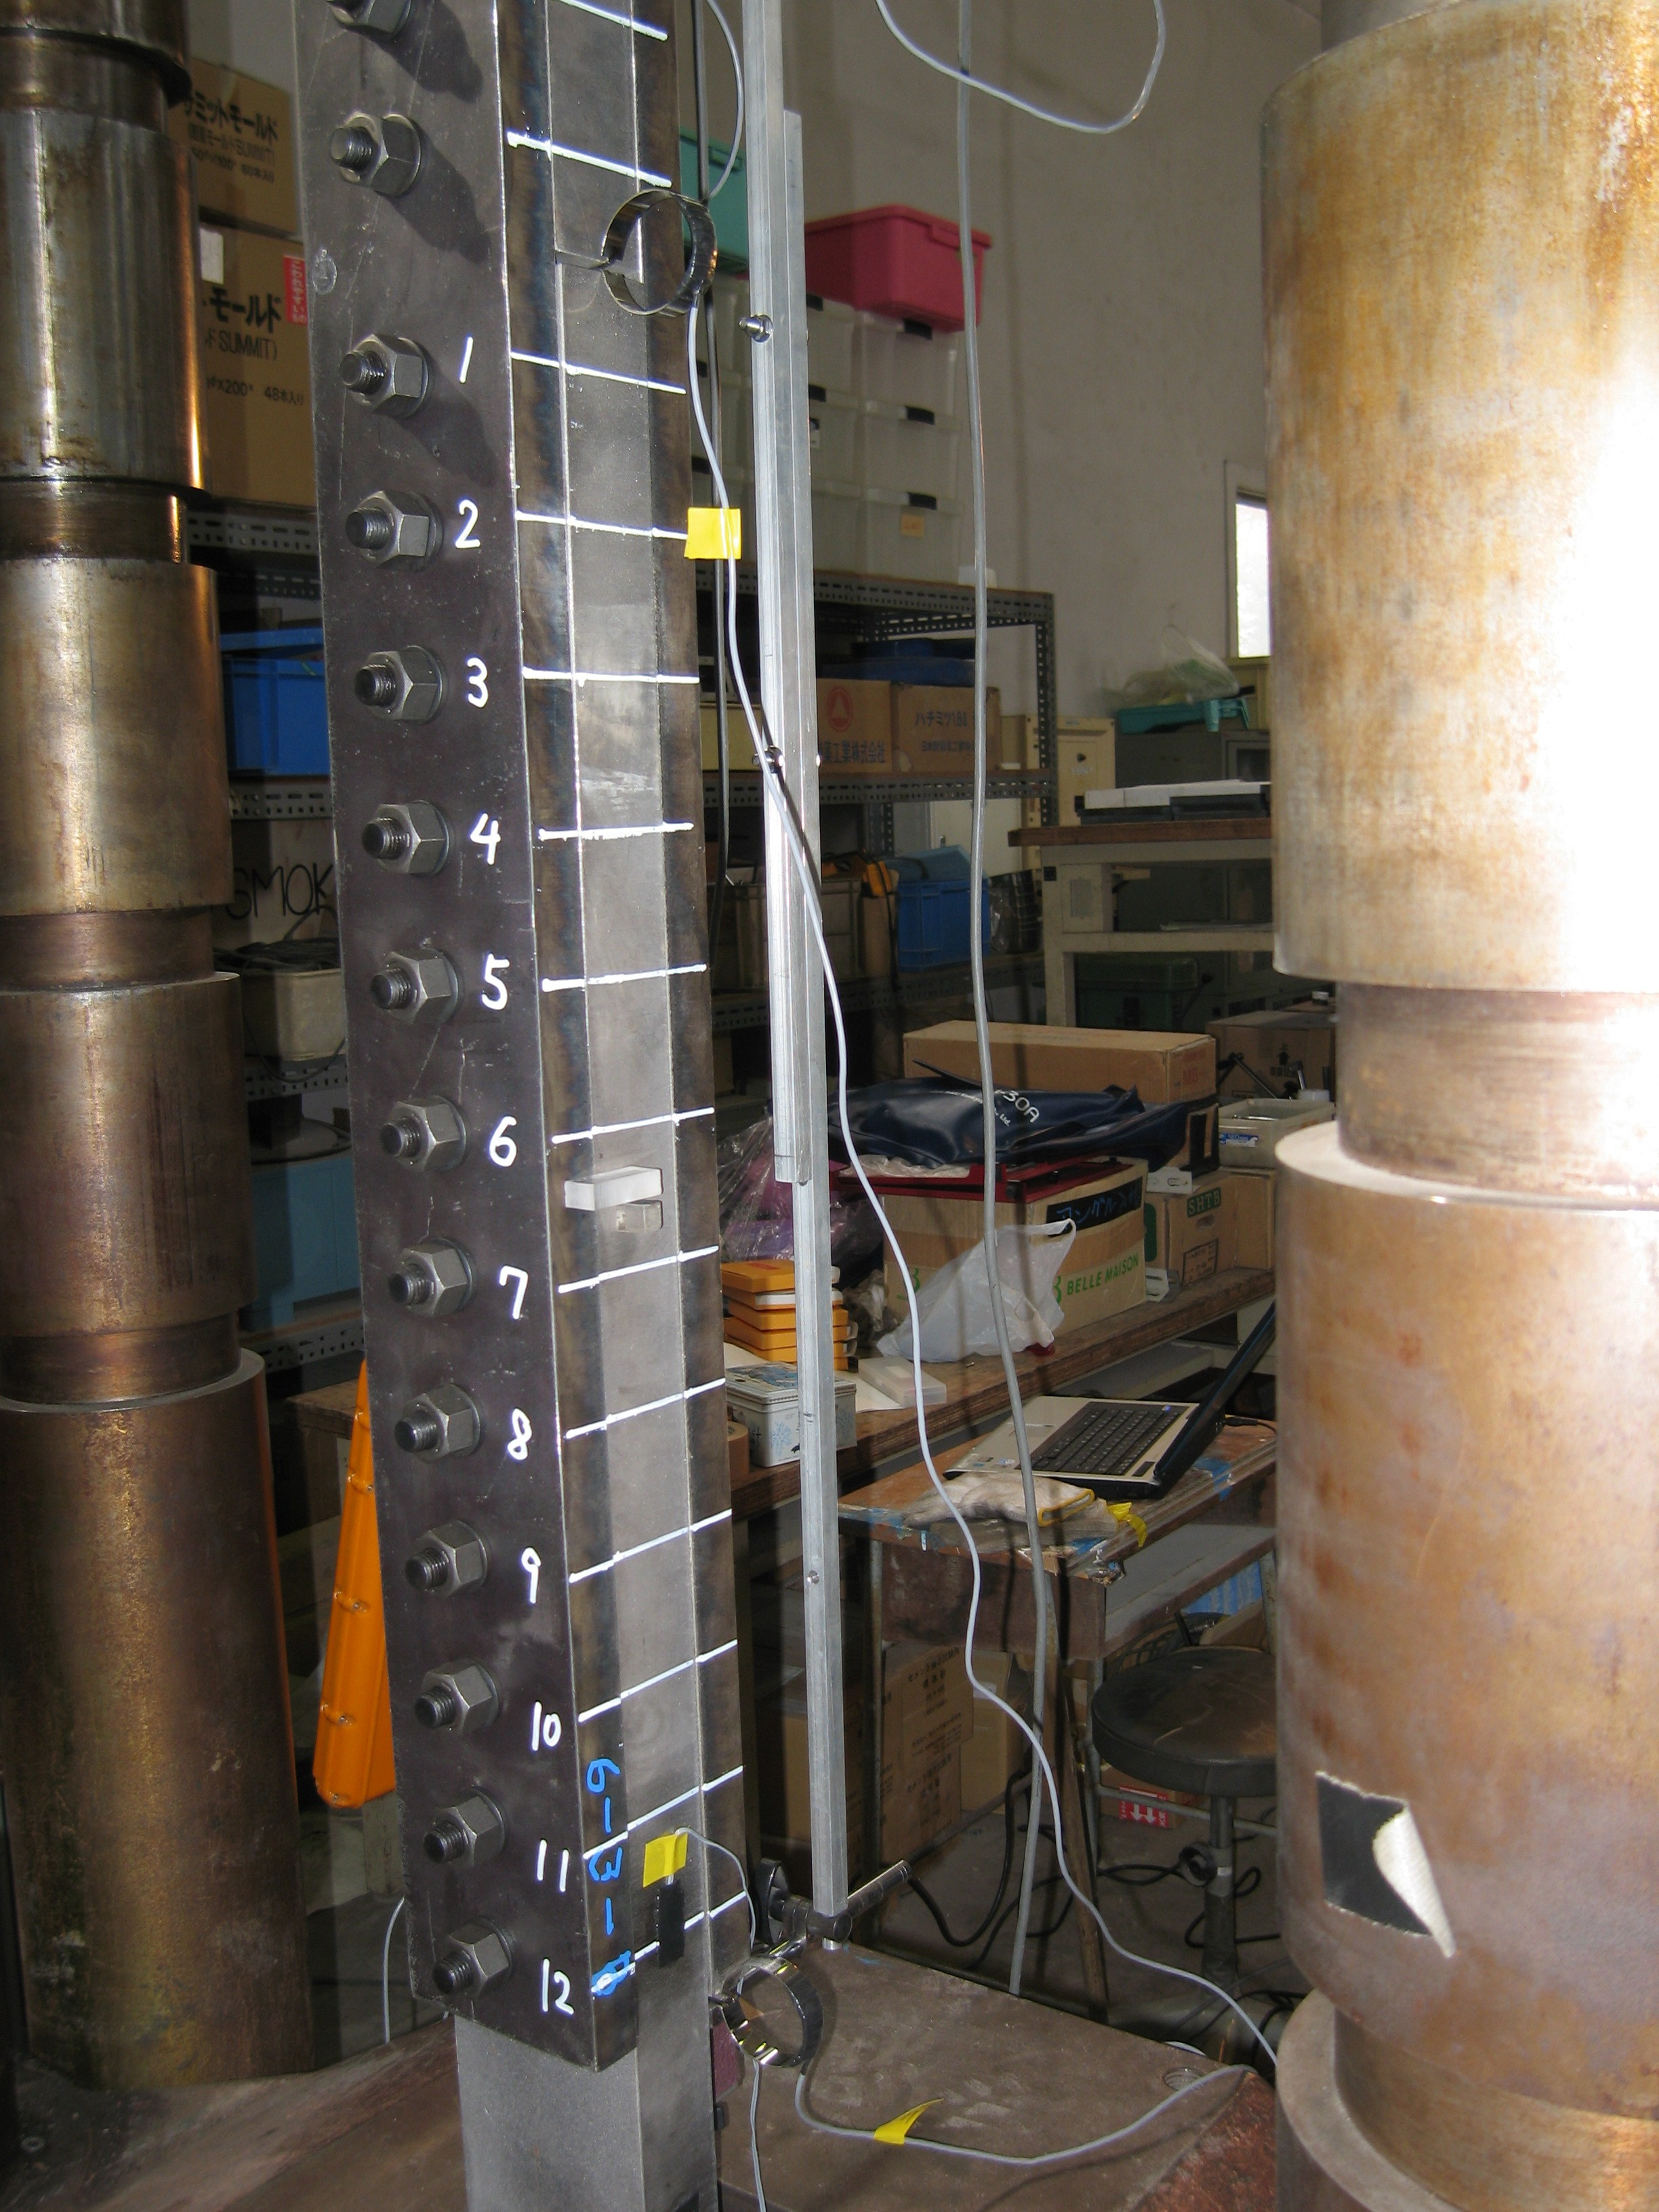
\includegraphics[width=\linewidth]{imgs/ch5/12rowtestpic.png}
        \caption{Setup of 12-row test specimen}
        \label{fig-testset}
    \end{subfigure}
    \hfill
    \begin{subfigure}[t]{0.55\textwidth}
        \centering
        \includegraphics[width=\linewidth]{imgs/ch5/validation.pdf}
        \caption{Validation of analysis model}
        \label{fig-validloadrd}
    \end{subfigure}
    \caption{Aging condition of rivet}
\end{figure}
\subsection{Analytical cases}
The analysis cases and bolt arrangements for each case are listed in Table \ref{tab-feboltarra}. Based on the investigation conducted in previous research \cite{kameilong}, it has been found that the majority of long joints consist of a row of bolts ranging from 8 to 12 in steel bridges. This study focuses on long bolted joints with 8 to 12 bolts, which are most prevalent in construction examples. A slip-critical bolted joint with 12 bolts has been established as the original case. 

To investigate the load-transfer mechanism and load-carrying capacity of the hybrid joints, we set the bolt arrangement (location and number of Interference-body bolts and High-strength hexagon bolts) and with or without Interference-body bolt preload as the analysis parameters. \par  
where the naming rule is as follows (for example, R12B1\#1 indicates that one Interference-body bolt was located at bolt position \#1 in the 12-row joint. R10B2 is the case where Interference-body bolts are arranged at outer \#1 and inner \#12 in the 10-row joint.):

\begin{tabular}{lp{6cm}}
    R\{number\} &  the number of bolts \\
    O &  the Original case \\
    B\{number\} &  the number of Interference-body bolt \\
    \#1 & the position of Interference-body bolt\\
    -NCF & Interference-body bolt without preload\\
%    mark t &   the thinckness of main plate\\
%    mark p &   the spacing of bolt\\
%    mark e &  the edge distance from end bolt\\
\end{tabular}

\begin{sidewaystable}[htbp]
\centering
\caption{ Bolt arrangement of FE model case}
\label{tab-feboltarra}
\scalebox{1.1}{
\begin{tabular}{@{}lcccccccccccccc@{}}
\toprule
\multirow{2}{*}{Case name}
 & \multicolumn{12}{c}{Fastener number} 
 & \multirow{2}{*}{\begin{tabular}[c]{@{}c@{}}preload of \\ Interference-body bolts\end{tabular}} 
 &\multirow{2}{*}{\begin{tabular}[c]{@{}c@{}}$\beta$ \\ $F_{ds}/F_{dy}$\end{tabular}} \\ \cmidrule(lr){2-13}
 & \multicolumn{1}{l}{\#1} & \multicolumn{1}{l}{\#2} & \multicolumn{1}{l}{\#3} & \multicolumn{1}{l}{\#4} & \multicolumn{1}{l}{\#5} & \multicolumn{1}{l}{\#6} & \multicolumn{1}{l}{\#7} & \multicolumn{1}{l}{\#8} & \multicolumn{1}{l}{\#9} & \multicolumn{1}{l}{\#10} & \multicolumn{1}{l}{\#11} & \multicolumn{1}{l}{\#12}  &\\ \midrule
 
R12-O  &\faCircleO&\faCircleO&\faCircleO&\faCircleO&\faCircleO&\faCircleO&\faCircleO&\faCircleO&\faCircleO&\faCircleO&\faCircleO&\faCircleO &205 kN &0.83\\
R12B1\#1 & \faGear&\faCircleO&\faCircleO&\faCircleO&\faCircleO&\faCircleO&\faCircleO&\faCircleO&\faCircleO&\faCircleO&\faCircleO&\faCircleO& 205 kN &0.83\\
R12B1\#1-NCF & \faGear&\faCircleO&\faCircleO&\faCircleO&\faCircleO&\faCircleO&\faCircleO&\faCircleO&\faCircleO&\faCircleO&\faCircleO&\faCircleO& 0 kN & 0.76\\
R12B1\#6 & \faGear&\faCircleO&\faCircleO&\faCircleO&\faCircleO&\faCircleO&\faCircleO&\faCircleO&\faCircleO&\faCircleO&\faCircleO&\faCircleO& 205 kN & 0.83\\
R12B1\#6-NCF & \faGear&\faCircleO&\faCircleO&\faCircleO&\faCircleO&\faCircleO&\faCircleO&\faCircleO&\faCircleO&\faCircleO&\faCircleO&\faCircleO& 0 kN & 0.76\\
R12B1\#12 & \faGear&\faCircleO&\faCircleO&\faCircleO&\faCircleO&\faCircleO&\faCircleO&\faCircleO&\faCircleO&\faCircleO&\faCircleO&\faCircleO& 205 kN & 0.83\\
R12B2 & \faGear &\faCircleO &\faCircleO&\faCircleO&\faCircleO&\faCircleO&\faCircleO&\faCircleO&\faCircleO&\faCircleO&\faCircleO&\faGear & 205 kN & 0.83\\
R12B2-NCF & \faGear &\faCircleO &\faCircleO&\faCircleO&\faCircleO&\faCircleO&\faCircleO&\faCircleO&\faCircleO&\faCircleO&\faCircleO&\faGear & 0 kN &0.69\\
R12B4 & \faGear & \faGear&\faCircleO&\faCircleO&\faCircleO&\faCircleO&\faCircleO&\faCircleO&\faCircleO&\faCircleO&\faGear  &\faGear  &  205 kN & 0.83 \\
R12B4-NCF & \faGear &  \faGear&\faCircleO&\faCircleO&\faCircleO&\faCircleO&\faCircleO&\faCircleO&\faCircleO&\faCircleO&\faGear  &\faGear  &   205 kN & 0.55\\
R12B12 &\faGear&\faGear&\faGear&\faGear&\faGear&\faGear&\faGear&\faGear&\faGear&\faGear&\faGear&\faGear& 205 kN & 0.83\\ 
R12B12-NCF &\faGear&\faGear&\faGear&\faGear&\faGear&\faGear&\faGear&\faGear&\faGear&\faGear&\faGear&\faGear& 205 kN & -\\ 
R10B0 & \faCircleO & \faCircleO & \faCircleO & \faCircleO & \faCircleO & \faCircleO & \faCircleO & \faCircleO & \faCircleO & \faCircleO &Null& Null& 205 kN & 0.69\\
R10B2 & \faGear & \faCircleO & \faCircleO & \faCircleO & \faCircleO & \faCircleO & \faCircleO & \faCircleO & \faCircleO & \faGear&Null&Null& 205 kN & 0.69\\
R10B4 & \faGear & \faGear & \faCircleO & \faCircleO & \faCircleO & \faCircleO & \faCircleO & \faCircleO & \faGear & \faGear&Null&Null& 205 kN &0.69\\
R8B0 & \faCircleO & \faCircleO & \faCircleO & \faCircleO & \faCircleO & \faCircleO & \faCircleO & \faCircleO &Null&Null&Null&Null&  205 kN & 0.55\\
R8B2 & \faGear & \faCircleO & \faCircleO & \faCircleO & \faCircleO & \faCircleO & \faCircleO & \faGear &Null&Null&Null&Null&  205 kN & 0.55\\
R8B4 & \faGear & \faGear & \faCircleO & \faCircleO & \faCircleO & \faCircleO & \faGear & \faGear &Null&Null&Null&Null&  205 kN & 0.55\\
\bottomrule
&&&\multicolumn{12}{r}{\faCircleO : High-strength hexagon bolt, \faGear : Interference-body bolt}
\end{tabular}}
\end{sidewaystable}


The FE cases are shown in Table \ref{tab-ch5fecase}. The parameters are the arrangement of bearing bolts and friction bolts and the presence or absence of axial force on the bearing bolts. The slip coefficient of -082 means 0.82.

\begin{table}[]
\centering
\caption{ Summary of FE analysis case and the parameter of each case}
\label{tab-ch5fecase}
\scalebox{0.8}{
\begin{tabular}{@{}lcccccccc@{}}
\toprule
\multicolumn{1}{c}{Case Name} &
  \begin{tabular}[c]{@{}c@{}}Thickness of\\ Main plate \\ $t $\\ $[mm]$\end{tabular} &
  \begin{tabular}[c]{@{}c@{}}Yield strength\\of Main plate\\ $\sigma_y$\\ $[Mpa]$\end{tabular} &
  \begin{tabular}[c]{@{}c@{}}Edge\\ Distance\\ $e_1$\\ $[mm]$\end{tabular} &
  \begin{tabular}[c]{@{}c@{}}Spacing of\\ Bolt\\ $p$\\ $[mm]$\end{tabular} &
  \begin{tabular}[c]{@{}c@{}}Number of \\ Bolt row\\ $N_b$\end{tabular} &
  \begin{tabular}[c]{@{}c@{}}Number of\\ B-bolt\\ $N_{Bb}$\end{tabular} &
  \begin{tabular}[c]{@{}c@{}}Preload of\\ B-bolt\\ $F_p$\\ $[kN]$\end{tabular} &
  \begin{tabular}[c]{@{}c@{}}$\beta$ \\ $F_{ds}/F_{dy}$\end{tabular} \\ \midrule
R12-O          & 75 & 365 & 40 & 75 & 12 & 0  & 205 & 0.83 \\
R12-B1\#1-NCF    & 75 & 365 & 40 & 75 & 12 & 1  & 0   & 0.76 \\
R12-B1\#1        & 75 & 365 & 40 & 75 & 12 & 1  & 205 & 0.83 \\
R12-B1\#6        & 75 & 365 & 40 & 75 & 12 & 1  & 205 & 0.83 \\
R12-B1\#6-NCF    & 75 & 365 & 40 & 75 & 12 & 1  & 0   & 0.76 \\
R12-B1\#12        & 75 & 365 & 40 & 75 & 12 & 1  & 205 & 0.83 \\
R12-B2         & 75 & 365 & 40 & 75 & 12 & 2  & 205 & 0.83 \\
R12-B2-NCF     & 75 & 365 & 40 & 75 & 12 & 1  & 0   & 0.76 \\
R12-B4         & 75 & 365 & 40 & 75 & 12 & 4  & 205 & 0.83 \\
R12-B4-NCF     & 75 & 365 & 40 & 75 & 12 & 4  & 0   & 0.55 \\
R12-B12        & 75 & 365 & 40 & 75 & 12 & 12 & 205 & 0.83 \\
R12-B12-NCF    & 75 & 365 & 40 & 75 & 12 & 12 & 0   & 0.83 \\
               &    &     &    &    &    &    &     &      \\
R12-O-t50-Bt1  & 50 & 420 & 40 & 75 & 12 & 0  & 205 & 1.08 \\
R12-B2-t50-Bt1 & 50 & 420 & 40 & 75 & 12 & 2  & 205 & 1.08 \\
R12-B4-t50-Bt1 & 50 & 420 & 40 & 75 & 12 & 4  & 205 & 1.08 \\
R10-B2-t50-Bt1 & 50 & 420 & 40 & 75 & 12 & 2  & 205 & 0.9  \\
R8-B2-t50-Bt1  & 50 & 420 & 40 & 75 & 12 & 2  & 205 & 0.72 \\
               &    &     &    &    &    &    &     &      \\
R12-O-p80   & 75 & 365 & 50 & 80 & 12 & 0  & 205 & 0.83 \\
R12-B2-p80  & 75 & 365 & 50 & 80 & 12 & 2  & 205 & 0.83 \\
R12-B4-p80  & 75 & 365 & 50 & 80 & 12 & 4  & 205 & 0.83 \\
R12-O-p85   & 75 & 365 & 50 & 85 & 12 & 0  & 205 & 0.83 \\
R12-B2-p85  & 75 & 365 & 50 & 85 & 12 & 2  & 205 & 0.83 \\
R12-B4-p85  & 75 & 365 & 50 & 85 & 12 & 4  & 205 & 0.83 \\
               &    &     &    &    &    &    &     &      \\
R12-O-Bt05*   & 75 & 420 & 40 & 75 & 12 & 0  & 205 & 0.53 \\
R12-O-p80Bt05* & 75 & 420 & 50 & 80 & 12 & 0  & 205 & 0.53 \\
R12-O-p85Bt05* & 75 & 420 & 50 & 85 & 12 & 0  & 205 & 0.83 \\
               &    &     &    &    &    &    &     &      \\
R10-Or         & 75 & 365 & 40 & 75 & 10 & 2  & 205 & 0.69 \\
R10-B2         & 75 & 365 & 40 & 75 & 10 & 2  & 205 & 0.69 \\
R10-B4         & 75 & 365 & 40 & 75 & 10 & 4  & 205 & 0.69 \\
R10-O-p80   & 75 & 365 & 50 & 80 & 10 & 4  & 205 & 0.69 \\
R10-B2-p80  & 75 & 365 & 50 & 80 & 10 & 4  & 205 & 0.69 \\
R10-B4-p80  & 75 & 365 & 50 & 80 & 10 & 4  & 205 & 0.69 \\
R10-O-p85   & 75 & 365 & 50 & 85 & 10 & 2  & 205 & 0.69 \\
R10-B2-p85  & 75 & 365 & 50 & 85 & 10 & 2  & 205 & 0.69 \\
R10-B4-p85  & 75 & 365 & 50 & 85 & 10 & 4  & 205 & 0.69 \\
               &    &     &    &    &    &    &     &      \\
R10-B2-420     & 75 & 420 & 40 & 75 & 10 & 2  & 205 & 0.6  \\
R10-B4-420     & 75 & 420 & 40 & 75 & 10 & 4  & 205 & 0.6  \\
               &    &     &    &    &    &    &     &      \\
R8-Or          & 75 & 365 & 40 & 75 & 8  & 2  & 205 & 0.55 \\
R8-B2-082      & 75 & 365 & 40 & 75 & 8  & 2  & 205 & 0.55 \\
R8-B4-082      & 75 & 365 & 40 & 75 & 8  & 4  & 205 & 0.55 \\
R8-Or-p80   & 75 & 365 & 50 & 80 & 8  & 2  & 205 & 0.55 \\
R8-B2-p80   & 75 & 365 & 50 & 80 & 8  & 2  & 205 & 0.55 \\
R8-B4-p80   & 75 & 365 & 50 & 80 & 8  & 4  & 205 & 0.55 \\
R8-Or-p85   & 75 & 365 & 50 & 85 & 8  & 2  & 205 & 0.55 \\
R8-B2-p85   & 75 & 365 & 50 & 85 & 8  & 2  & 205 & 0.55 \\
R8-B4-p85   & 75 & 365 & 50 & 85 & 8  & 4  & 205 & 0.55 \\ \bottomrule
\end{tabular}}
\clearpage
\end{table}

\subsection{Strength of the joint}
The design strength of the original case (R12-O) is presented in Fig. \ref{tab-strength}. To investigate the load-sharing state and mechanical behavior of a single bolt, the load-carrying capacity (slip, bearing, and shear capacities) per bolt was calculated using Eqs. (\ref{eq-fds1}–\ref{eq-fdsy1}), and the design strength of the entire bolted joint is calculated using Eqs.(\ref{eq-fdy}–\ref{eq-fdsy}), respectively. \par
Because the reduction factor of the joint length and judgment of slip between Japan and Europe were different, this study was not considered for ease of slip strength evaluation. The assessment of slip is a 0.2 mm relative displacement, as mentioned in Section 2.2.

\noindent Slip resistance per a fastener:
\begin{equation}
    \label{eq-fds1}
    F_{ds1} = \mu \times N \times m
\end{equation}

Bearing resistance per fastener
\begin{equation}
    \label{eq-fdb1}
    F_{db1} = 1.5 \times \sigma_y \times t \times d_b
\end{equation}

Bolt-shank shear yield resistance per fastener
\begin{equation}
    \label{eq-fdsy1}
    F_{dsy1} = \sigma_{yb} / \sqrt{3} \times 2 \pi \times (0.5d_b)^2
\end{equation}
Net cross-sectional yield strength of the plate
\begin{equation}
    \label{eq-fdy}
    F_{dy} = (w-d_0)t \times \sigma_y
\end{equation}
Ultimate tensile strength of the plate
\begin{equation}
    \label{eq-fdu}
    F_{du} = (w-d_0)t \times \sigma_u
\end{equation}
Slip Strength (Total)
\begin{equation}
    \label{eq-fds}
    F_{ds} = F_{ds1} \times n_{f}
\end{equation}
Bolt-shank shear yield strength (total)
\begin{equation}
    \label{eq-fdsy}
    F_{dsy} = F_{dsy1} \times n
\end{equation}

where $\sigma_y$ and $\sigma_u$ are the yield and ultimate strengths of the main plate, respectively; $t$ is the thickness of the main plate; $\mu$ is the slip coefficient; $N$ is the preload of the bolts; $m$ is the number of shear planes; $d_b$ is the diameter of the bolt; $\sigma_{yb}$ is the yield strength of the HSB; $w$ is the width of the main plate; $d_0$ is the hole diameter; $n_{f}$ is the number of High-strength hexagon bolts; and $n_b$ is the number of Interference-body bolts.

\begin{table*}[ht]
    \centering
    \caption{ Design resistance of Original case (R12-O, $\beta$: 0.83. unit: kN)}
    \label{tab-strength}
    \begin{tabular}{@{}ccccccc@{}}
    \toprule
      \multicolumn{3}{c}{Resistance per fastener} &
      \multirow{2}{*}{\begin{tabular}[c]{@{}c@{}}Cross-section\\ yield strength\\ $F_{dy}$\end{tabular}} &
      \multirow{2}{*}{\begin{tabular}[c]{@{}c@{}}Ultimate tensile\\  strength\\ $F_{du}$\end{tabular}} &
      \multirow{2}{*}{\begin{tabular}[c]{@{}c@{}}Slip \\ strength\\ $F_{ds}$\end{tabular}} &
      \multirow{2}{*}{\begin{tabular}[c]{@{}c@{}}Shear yield \\ strength\\ $F_{dsy}$\end{tabular}} \\ \cmidrule(r){1-3}
    \begin{tabular}[c]{@{}c@{}}Slip \\ resistance*\end{tabular} &
      \begin{tabular}[c]{@{}c@{}}Bearing \\ resistance*\end{tabular} &
      \begin{tabular}[c]{@{}c@{}}Shear yield \\ resistance*\end{tabular} &       &       &       &
       \\ \midrule
    164 &  972.9 & 450.76 &  2367.9 &     3535.7 &  1968 &  5409.1 \\ \bottomrule
    \end{tabular}
\end{table*}

%%%%%%%%%%%%%%%%%%%%%%%%%%%%%%%%%%%%%%%%%%%%%%%%%%%%%%%%%%%%
%%%%%%%% Result
%%%%%%%%%%%%%%%%%%%%%%%%%%%%%%%%%%%%%%%%%%%%%%%%%%%%%%%%%%%%
\section{Results and discussions}

\subsection{Displacement of hybrid joint}


%%%
%Slip strength with Eurocode3 or ASSHTO evaluate the relative displacement of each location(10mm,center of joint and end of joint) %deformation of net cross-section when end bolt is bearing-type (effict, where is different.) transfer mechanism 
%%%

The relationship between the load and deformation of the joint is shown in Fig. \ref{fig-loadD}, where deformation is taken from the joint end located at the applied load. The relationship between the load and relative displacement is shown in Fig. \ref{fig-loadrd}. Relative displacement is referenced to the AIJ's \cite{AIJ2012AIJStructures} recommendation and taken from the location of distance 10 mm from the inner end of the plate. Peng et.al \cite{Peng2013FeaDimensions} investigated the correctness of a 0.2 mm relative displacement slippage estimation for long-bolted joints. In Fig. \ref{fig-loadD}, the square represents the R12-o case (original slip-critical bolted joint), the circle represents a hybrid joint with two Interference-body bolts, and the triangle represents a hybrid joint with four Interference-body bolts. The dash-dotted line $F_{ds}$ and dashed line $F_{dy}$ represent the design slip strength and net cross-sectional yield strength of the R12-o case, respectively.

\begin{figure}[htbp]
    \begin{subfigure}[t]{0.49\textwidth}
        \centering
        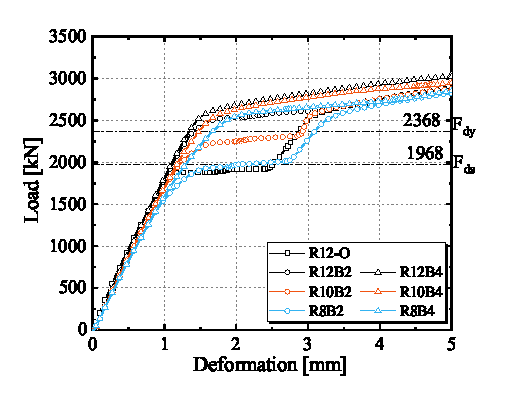
\includegraphics[width=\linewidth]{imgs/ch5/LD-A.eps}
        \caption{Relationship between load and deformation of joint}
        \label{fig-loadD}
    \end{subfigure}
    \begin{subfigure}[t]{0.49\textwidth}
        \centering
        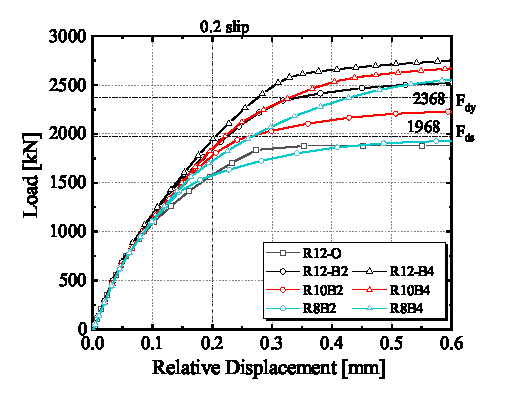
\includegraphics[width=\linewidth]{imgs/ch5/load-rd.eps}
        \caption{Relationship between load and relative displacement}
        \label{fig-loadrd}
    \end{subfigure}
\end{figure}


The case arranged with two Interference-body bolts (R8B2, R10B2) occurred twice with significant changes in slope. Here, ``slip'' had occurred with a slip-critical bolted joint, as shown in Fig. \ref{fig-loadD}. This was owing to the shear plastic deformation of the end-Interference-body bolt shank, which caused the joint to slip as a whole. 

As shown in Fig. \ref{fig-loadrd}, before the original case (R12-O) reaches the designed slip strength (1968 kN), the joint undergoes \ac{Major slip} (1858 kN) owing to the unbalance of load distribution, and the 0.2 mm slip load decreased to 1,594 kN. The major and 0.2 mm slip loads were reduced by approximately 6\% and 19\%, respectively, relative to the designed slip strength. However, for the B2 case with Interference-body bolts arranged, load decrease did not occur, and a nonlinear change in the curve occurred at approximately 2,387 kN. This change in slope was due to the cross-sectional yield. A major slip is defined as when the slope of the load-relative displacement curve decreases to near horizontal and is maintained until the friction bolt enters the bearing state. 

The R12B4 hybrid joint exhibited the highest load compared with another case at relative displacements up to 0.2 mm, followed by R12B2 and R10B4; R10B2, R12-O, and R8B2 had the lowest loads. These results suggest that increasing the number of Interference-body bolts at each end can significantly improve the slip strength, even if the joint length is shortened to 10 or 8 rows, while maintaining the same cross-sectional configuration.

In addition, R10B2 and R8B2 exhibit almost the same slope change trend, as shown in Fig. \ref{fig-loadrd}. Although the slope was decreased (except the horizontal as mentioned above), their change in displacement and slope can be interpreted as being due to bolt-shank plastic deformation. 

 Considering the initial slope shown in Fig. \ref{fig-loadrd}, it can be found that because of the local slip of the bolts arising from the ``unbuttoning'' phenomenon, the slope of the original case gradually decreases. 

\subsection{Relative displacement distribution of entire joint}

\begin{figure}[htbp]
\centering
    \begin{subfigure}[t]{0.49\textwidth}
        \centering
        \includegraphics[width=\linewidth]{imgs/ch5/re-eabt-02.eps}
        \caption{When tensile force = 0.2 mm slip load}
        \label{fig-f02rdd}
    \end{subfigure}
    \hfill
    \begin{subfigure}[t]{0.49\textwidth}
        \centering
    \includegraphics[width=\linewidth]{imgs/ch5/re-eabt-ds.eps}
    \caption{When tensile force = designed slip strength (1,968 kN)}
    \label{fig-fdsrdd}
    \end{subfigure}
\caption{Relative  displacement of the main and splice plate distribution at each bolt for the entire joint (a. 0.2 mm slip load; b. Original case's Design slip load)}
\label{fig-rdd}
\end{figure}

Fig. \ref{fig-rdd} shows the relative displacement of the main and splice plate distribution at each bolt for the entire joint. Fig. \ref{fig-f02rdd} shows the relative displacement distribution when the tensile force reaches a 0.2 mm slip load. Fig. \ref{fig-fdsrdd} shows the relative displacement distribution when the tensile force reaches the design slip strength.

Although the 0.2 mm slip load of hybrid joint R12B2 is 1.13 times higher than that of the slip-critical joint, the relative displacement distribution is approximately identical, as shown in Fig. \ref{fig-f02rdd}. This is because neither joint experienced major slip. Only elastic deformation occurred from the end of the joint to the center, and the load was primarily transmitted by friction. The hybrid joint can be designed similar to a slip-critical joint.

When the tensile force reached the design slip strength (1,968 kN), each bolt location in the slip-critical joint exhibited a major relative displacement. Conversely, the R12B2 hybrid joint remained at a low relative displacement, and a 0.01 mm relative displacement was achieved  at the \#6 bolt location, which is the center of the joint, as shown in Fig. \ref{fig-fdsrdd}. For slip design, owing to the presence of a Interference-body bolt, the hybrid joint can ignore the reduction in slip strength of the long-bolted joint.

\subsection{Load distribution}

The load distributions of the bolts for R12-O, R12-B2, R8B2, and R8B4 are shown in Fig. \ref{fig-load3d}. The x-axis in the Figure represents the bolt number, y-axis represents the resistance shared by each bolt, and z-axis represents the overall tensile force on the joint. The shaded plane represents the designed slip strength of one bolt ($F_{ds1}=164 $ kN), where the slip resistance is the total force calculated by the shear stress of the top surface in the main plate, the bearing resistance is the total force calculated by the sum of the contact pressure of the hole surface, and the tensile force is equal to the sum of the bearing resistance and slip resistance of each bolt, as shown in Fig. \ref{fig-how2cal-resis}. 

When the load exceeded 500 kN, owing to the deformation of the main plate, the plate thickness decreased, end bolt \#1 had a load of 143 kN, and the load was no longer transferred, resulting in a localized slip, as shown in Fig. \ref{fig-r12o3d}. A local slip occurred in the joint in sequence from the end bolt to the inner bolt (i.e., \#1 to \#6). Because slipped bolts do not transmit more load until they enter the bearing, the ability of the joints to transmit load is reduced. This explains the nonlinear change in the initial slope of the relative displacement and its continuous decrease, as shown in Fig. \ref{fig-loadrd}.

In contrast, hybrid joints with Interference-body bolts ( Fig. \ref{fig-r12b23d}, \ref{fig-r8b23d}, and \ref{fig-r8b43d}) continue to transfer load through bearing, thanks to the outermost Interference-body bolt, even if the contact interface is no longer able to resist additional friction forces. Thus, the joint could bear the load as a whole.

In addition, owing to the yielding of the net cross-section, the plate thickness decreased and caused a reduction in the bolt axial force. Therefore, the end ends \#1, \#2, \#11, and \#12 (or \#7, \#8) High-strength hexagon bolt in Fig. \ref{fig-load3d} have a significant decrease in resistance of one bolt. The end-Interference-body bolt did not exhibit an obvious decrease in force because the bearing bolt transmitted loads primarily in a bearing and shear manner. The decrease in the resistance of one bolt can be neglected because the friction force caused by the Interference-body bolt was not included in the strength calculation.

%3D Fig
\begin{figure}[htbp]
\centering
    \begin{subfigure}[t]{0.49\linewidth}
        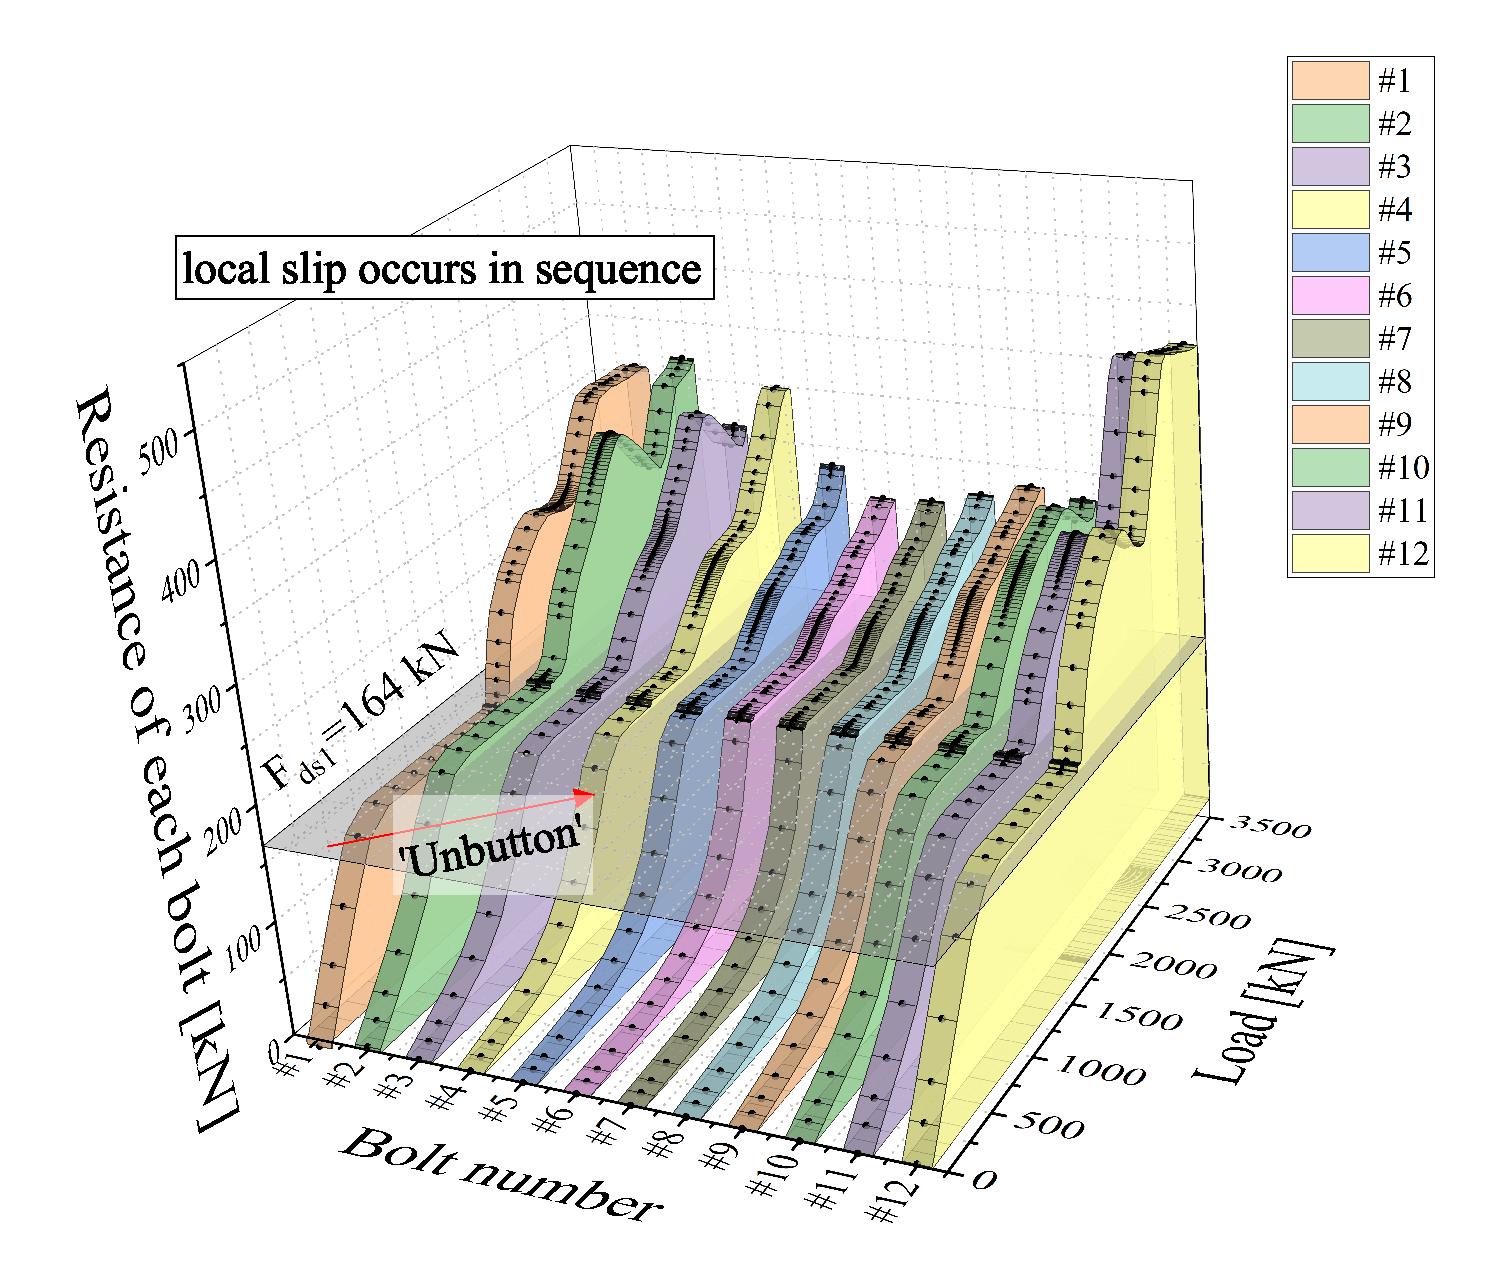
\includegraphics[width=\linewidth]{imgs/ch5/R12-O-3d.eps}
        \caption{R12-O case}
        \label{fig-r12o3d}
    \end{subfigure}
    \hfill
    \begin{subfigure}[t]{0.49\linewidth}
        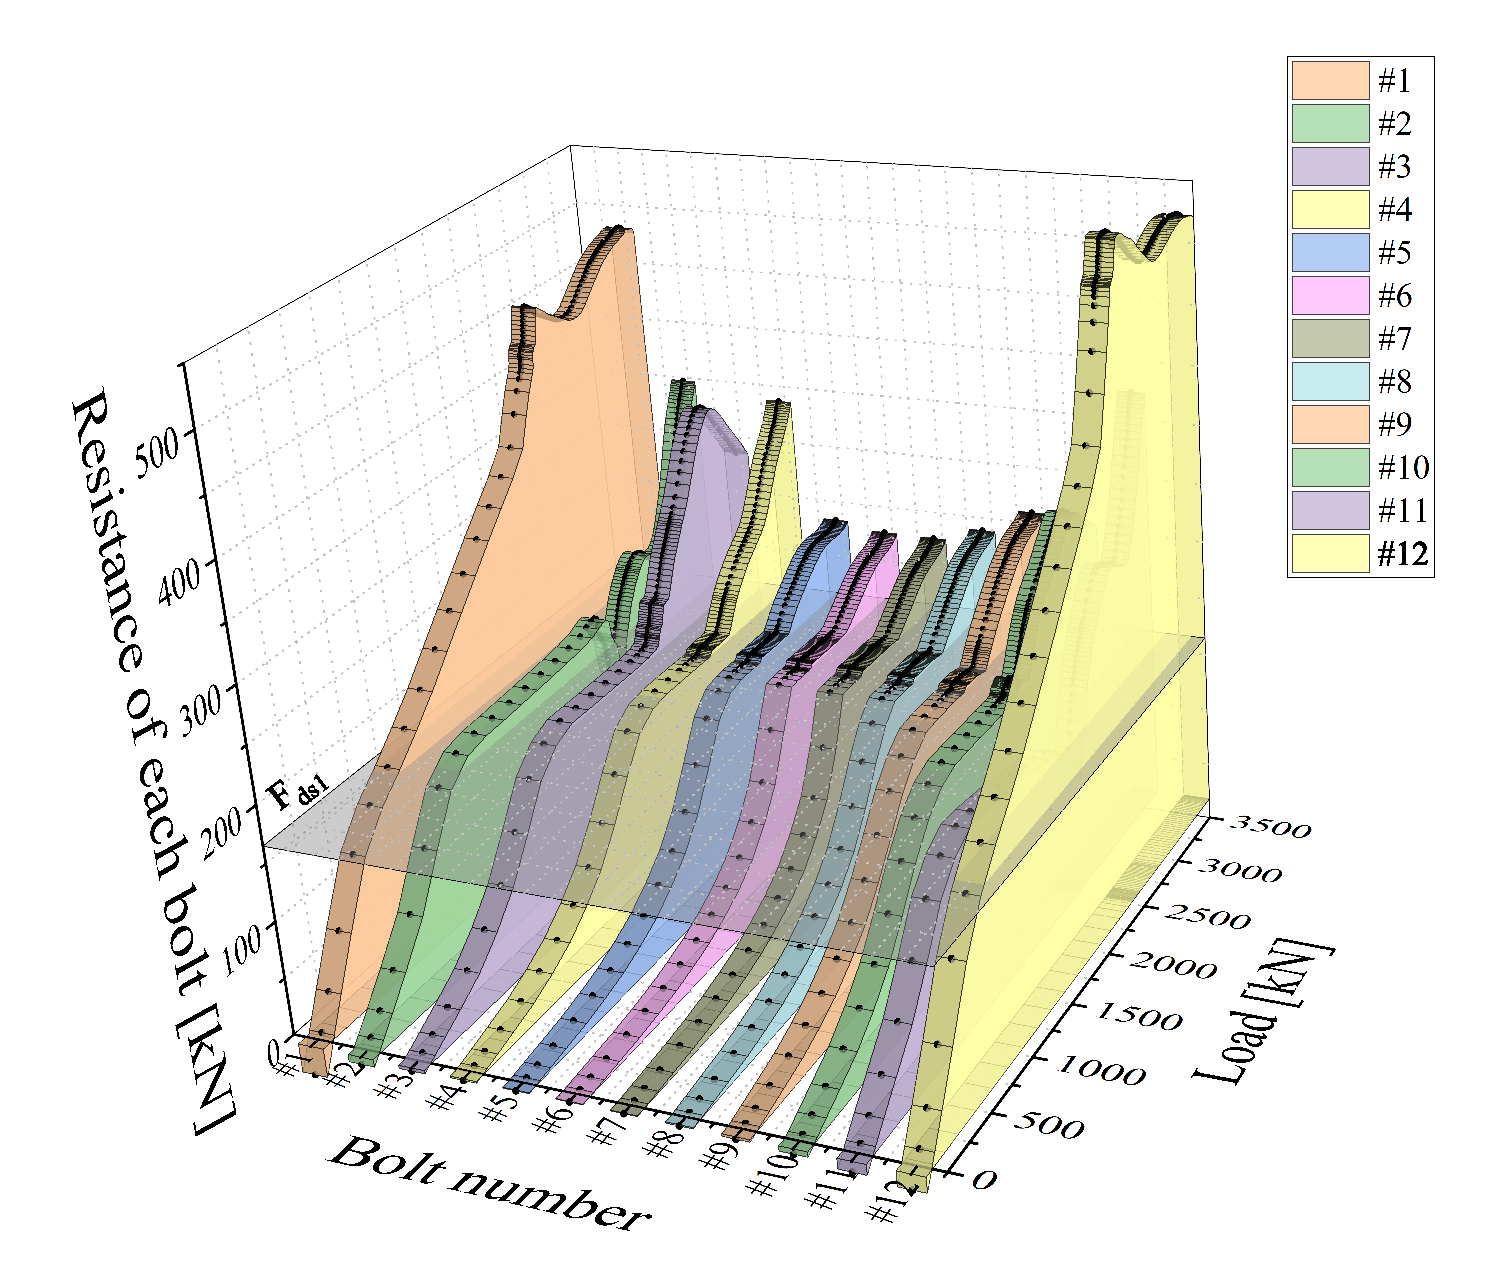
\includegraphics[width=\linewidth]{imgs/ch5/R12B2--3d.eps}
        \caption{R12-B2 case}
        \label{fig-r12b23d}  
    \end{subfigure}
    \hfill
    \begin{subfigure}[t]{0.49\linewidth}
        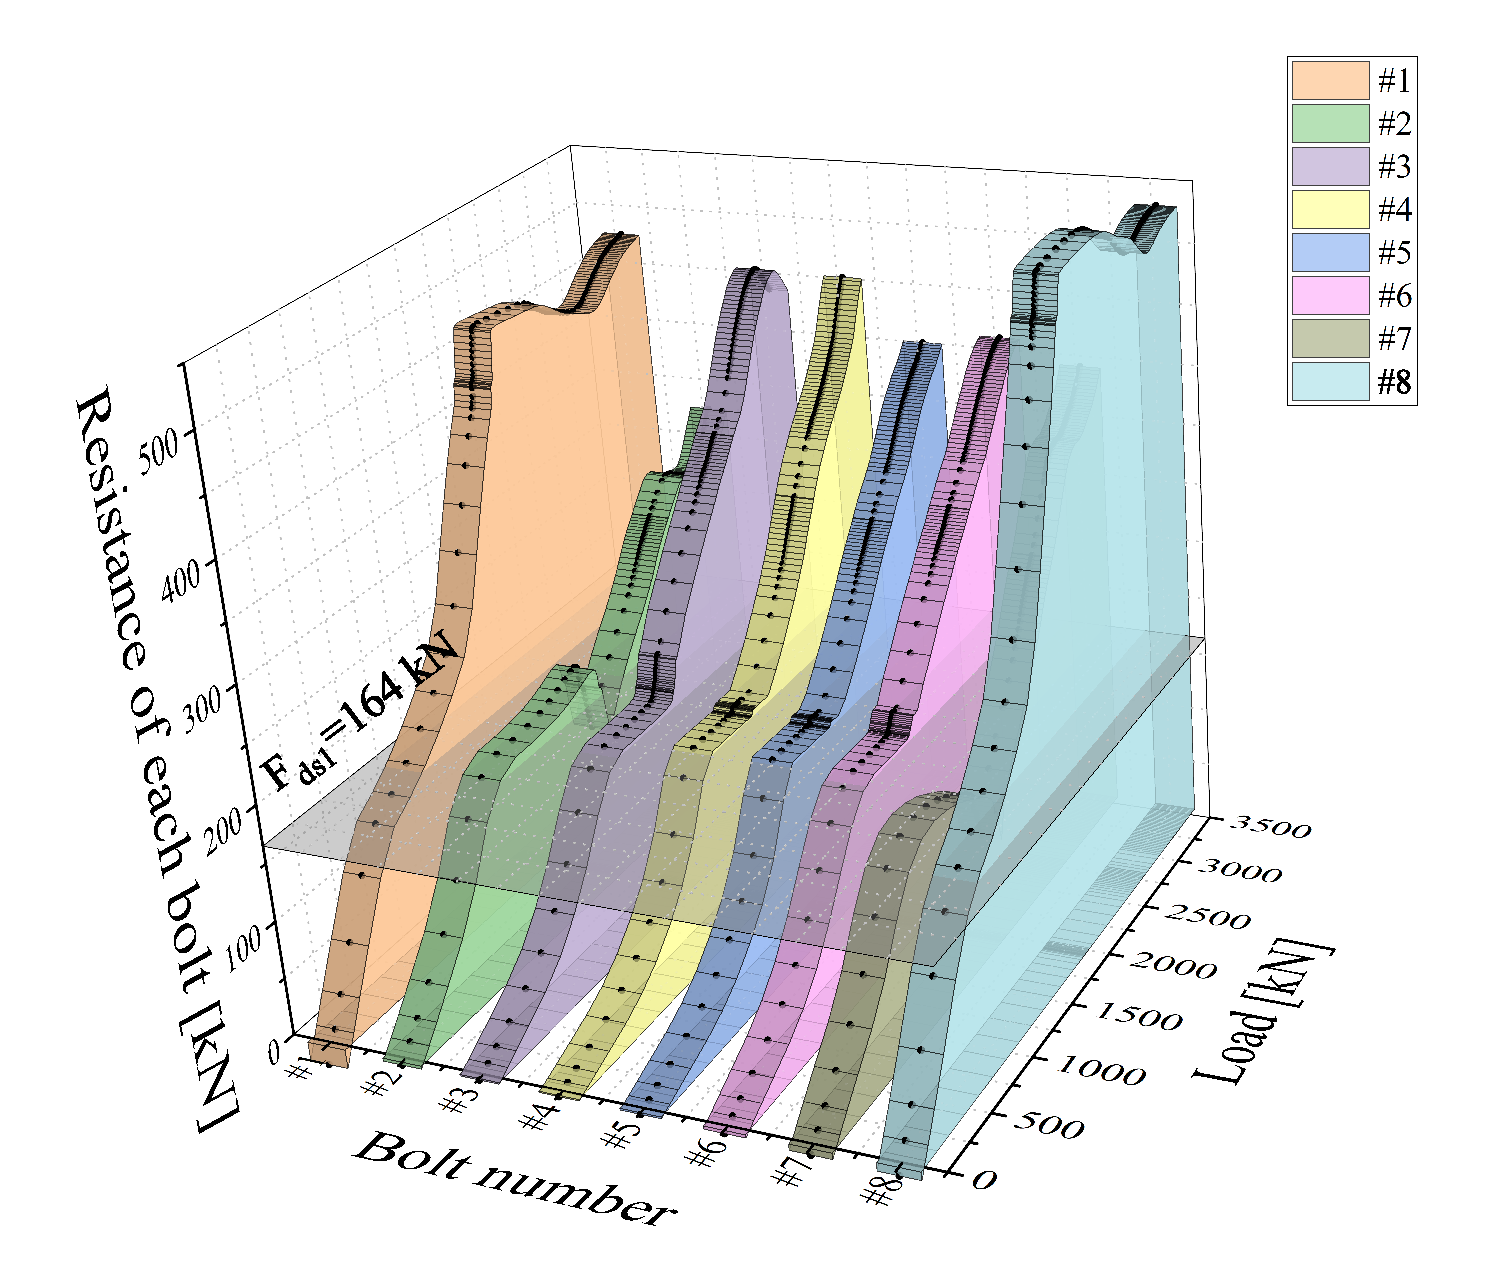
\includegraphics[width=\linewidth]{imgs/ch5/R8B2-3d.eps}
        \caption{R8B2 case}
        \label{fig-r8b23d}
    \end{subfigure}
    \hfill
    \begin{subfigure}[t]{0.49\linewidth}
        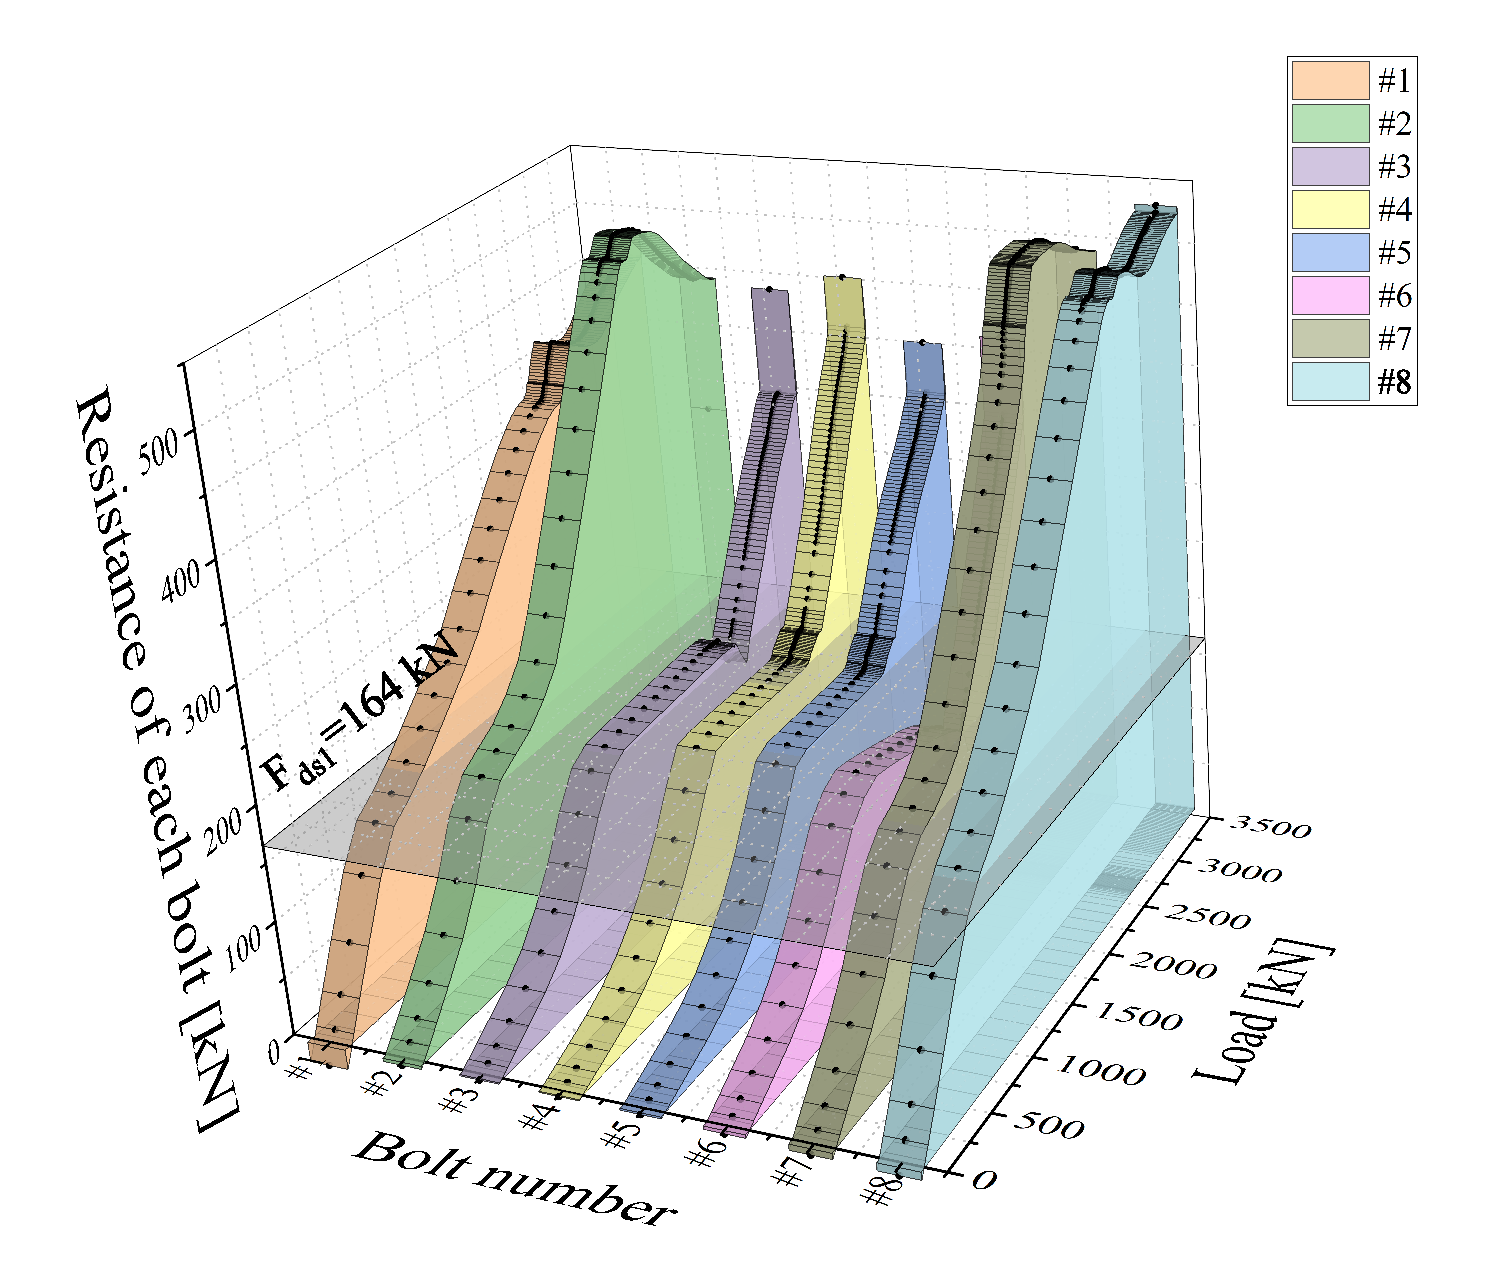
\includegraphics[width=\linewidth]{imgs/ch5/R8B4-3d.eps}
        \caption{R8B4 case}
        \label{fig-r8b43d}  
    \end{subfigure}
\caption{Relationship between Resistance of each bolt, Bolt number and Load.}
\label{fig-load3d}
\end{figure}

\begin{figure}[htbp]
    \centering
    \includegraphics[width=0.95\linewidth]{imgs/ch5/how2cal-resis.pdf}
    \caption{Calculate method of friction / bearing resistance of each bolt}
    \label{fig-how2cal-resis}
\end{figure}

\begin{figure}[htbp]
    \begin{subfigure}[t]{0.49\textwidth}
      \centering
      \includegraphics[width=\linewidth]{imgs/ch5/R12BSratio-FSS.eps}
      \caption{R12 case}
      \label{fig-bsharer12}
    \end{subfigure}
    \hfill
    \begin{subfigure}[t]{0.49\textwidth}
      \centering
      \includegraphics[width=\linewidth]{imgs/ch5/R10BSratio-FSS.eps}
      \caption{R10 case}
      \label{fig-bsharer10}
    \end{subfigure}
    \hfill
    \begin{subfigure}[t]{\linewidth}
      \centering
      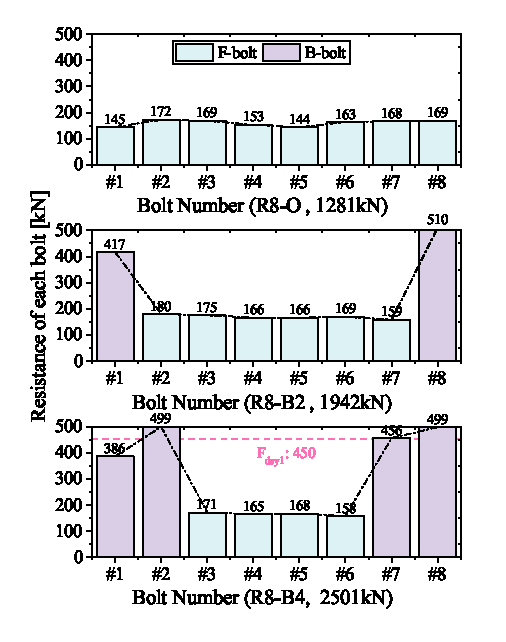
\includegraphics[width=0.49\linewidth]{imgs/ch5/R8BSratio-FSS.eps}
      \caption{R8 case}
      \label{fig-bsharer8}
    \end{subfigure}
\caption{Resistance of each bolt when load when the case is SLS}
\label{fig-bshare}
\end{figure}

Fig. \ref{fig-bshare} shows the load-share distribution of each bolt at the hybrid joint with SLS. where the blue bar represents High-strength hexagon bolt; purple bar represents Interference-body bolt. when the slip-critical joint (R12-O, R10-O) experienced major slip, the inner bolt (i.e., \#5 \#6, \#7 bolt in R12-O) could not develop the maximum friction they could resist (164 kN), and the resistance of the end bolt was also reduced by the deformation of the main plate. Therefore, a long slip-critical joint cannot reach the design slip strength. However, for a hybrid joint (e.g., R12B2), where the SLS is the bolt-shank shear yield or net cross-section yield, when the joint reaches SLS, all the inner High-strength hexagon bolt transmit almost the same amount of force (i.e., the maximum friction that they can resist). 

Furthermore, Fig.\ref{fig-bshare} illustrates that when using only one Interference-body bolt at each end of the hybrid joint (i.e. R12b2, R10b2), the Interference-body bolt transmits too much tensile load compared to the High-strength hexagon bolt. This caused the bolt shank to shear yield ($F_{dsy1}$ = 450 kN) before the net cross-sectional yield of the joint occurred. However, using two Interference-body bolts at each end evenly distributes the tensile load between the two bolts, allowing the joint to maintain its elasticity before experiencing a net cross-sectional yield.


\begin{figure}[htbp]
    \centering
    \includegraphics[width=0.9\linewidth]{imgs/ch5/r8b24misescs0-1940.png}
    \caption{von-Mises stress counter of R8B4 and R8B2 cases when tensile force = $P_{ss}$ (2242 kN)}
    \label{fig-r10b24boltmises}
\end{figure}

Fig. \ref{fig-r10b24boltmises} also shows the R10B4 and R10B2 case's von-Mises stress counter when tensile force equal to the bolt shear yield load for R8B2, end bolts' (\#1 and \#8) shear plane of R8B2 case occurs cross-section yield. For R8B4, the tensile forces originally concentrated on bolts \#1 and \#8 were distributed to the adjacent Interference-body bolts, resulting in a more even distribution of the bolt shear stresses and no yielding of the end Interference-body bolt.

Based on the above results, we recommend the installation of only one Interference-body bolt at each end in practical engineering design. This is because the Interference-body bolt may experience local shear yield before the joint experiences a net cross-sectional yield, which would reduce the load-bearing capacity of the joint. Therefore, to prevent an excessive tensile load on a single bolt, it is necessary to use at least two Interference-body bolts at each end of a long hybrid joint.

\textbf{Load sharing of the end bolt}

The relationship between the load-bearing force of the bolt at the end (\#1) and the load made non-dimensional by the slip resistance $F_{ds}$ is shown in Fig. \ref{fig-load-non-1bs}. The relationship between the load/$F_{ds}$ and the resistance of each bolt / total load is shown in Fig. \ref{fig-load-1bs-alnon}. As shown in Fig. \ref{fig-load-non-1bs}, only the friction force of the R12-O bolt reaches its designed value at about 150 kN, causing localized slip in the friction joint. This is considered to be a reduction of preload due to $\beta$. All of cases, before $F_{ds1}$ is reached, the slope of the load sharing curves for the same number of rows of bolts coincides. This suggests that friction force is dominant for bearing type bolts before $F_{ds1}$ is reached. The slope of the load sharing curve changes around $F_{ds1}$, and the load is resisted by both friction and bearing. Fig. \ref{fig-load-1bs-alnon} shows a non-dimensionalized view of the load-sharing force of the bolts. Regardless of the number of rows, when the load is equal to the design slip resistance $F_{ds}$ for any of the hybrid joints, the \#1 bolts at the ends carry approximately 17\% of the load. In all cases except for the case where no preload is introduced, the load on the end bolts decreases after reaching 27\%.

\begin{figure}[htbp]
\begin{minipage}[t]{0.49\linewidth}
    \centering
    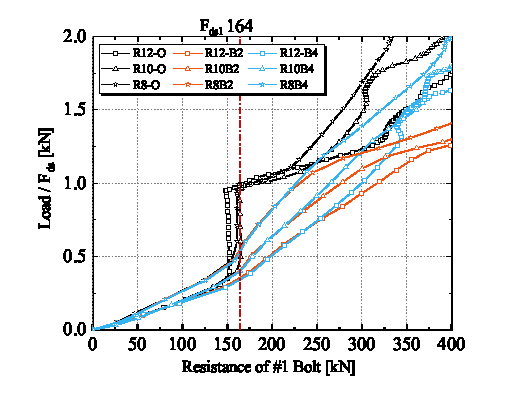
\includegraphics[width=\linewidth]{imgs/ch5/Load-non-1BS.eps}
    \caption{Relationship between load with Nondimensionalization by design slip strength and the resistance of $\#1$ bolt}
    \label{fig-load-non-1bs}
\end{minipage}
\hspace{0.01\textwidth}
\begin{minipage}[t]{0.49\linewidth}
    \centering
    \includegraphics[width=\linewidth]{imgs/ch5/Load-1BS-alnon.eps}
    \caption{Relationship between load with Nondimensionalization by design slip strength and the resistance of \#1 bolt Nondimensionalization by load}
    \label{fig-load-1bs-alnon}
\end{minipage}
\end{figure}

\subsection{Reduction of the slip load}

Fig. \ref{fig-bpreload-r8o} shows the friction resistance calculated from the actual preload of the bolt and the relationship between the load and the resisting force received by the \#1 bolt at the front end. The joint is elastically deformed by the tensile force due to the Poisson effect on the splice plate and the material to be jointed. As a result, the preload of the bolt also decreases, and the actual friction load is lower than the slip resistance $F_s$ calculated from the introduced preload $N$. Slip occurs when the resistance force of the bolts intersects the actual friction force. The greater the number of bolts, the greater the reduction in load when the main slip occurs in the joint.

\begin{figure}[htbp]
    \centering
    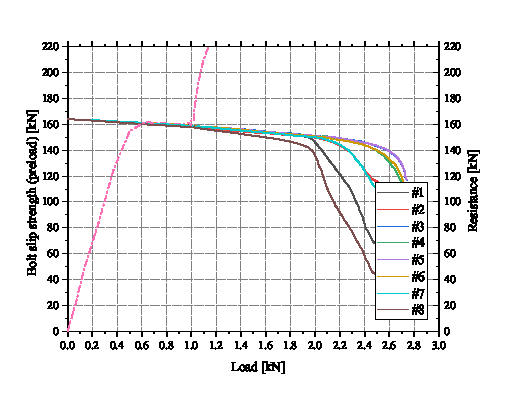
\includegraphics[width=0.7\linewidth]{imgs/ch5/bpreload-r8o.eps}
    \caption{The relationship between slip strength per Bolt(calculated by $N \times 2 \times 0.4$) and load (R8-O case)}
    \label{fig-bpreload-r8o}
\end{figure}

The relationship between the rate of reduction of sliding load and joint length for each case is shown in Fig. \ref{fig-fdsredu} .R12-bt06-Hou plots the experimental results of previous studies. In the R12-O case, the relationship between the joint length and the rate of reduction of slip load is almost consistent with Eurocode's equation for reduction of slip load, which is below the equation for reduction of slip load in the R12-O case, because the $\beta$ of R12-O is 0.8, indicating the effect of net section yielding.

\begin{figure}[htbp]
    \centering
    \includegraphics[width=0.75\linewidth]{imgs/ch5/F02-Fds-L-eq-new.eps}
    \caption{The relation ship of Reduction of slip strength(the ratio of 0.2mm slip strength to design slip strength) and Joint length}
    \label{fig-fdsredu}
\end{figure}

\subsection{Discussion of bearing critical of hybrid-bolted joint at SLS}

The slip-critical joint was defined as having two SLSs: slip-critical and net cross-section yield critical states. Kamei et al. \cite{kamei2010} considered that the bearing joint could use the same design method as the slip-critical joints. A previous study indicated that the bearing deformation limit could be used \cite{Rex2003,TODA2014} as the SLS of the bearing joint. The relative displacement of the hybrid joint was limited by the bearing manner. We consider that the hybrid joint would not occur a major slip, but it would occur significant deformation like ``slip'' due to the bolt-shank shear yield or bearing deformation of steel plate.

However, for the hybrid joint, based on the results above, we know that because the Interference-body bolt is arranged at the end of the joint, which has the highest load share, the Interference-body bolts will share more tensile force than the inner High-strength hexagon bolt, and the internal High-strength hexagon bolt performed better before the joint moved to the plastic state. Therefore, one of the purposes of the hybrid joint is to make as many friction bolts as possible within the bearing strength of end fit bolts.

This analysis defined the \ac{Bolt shear yield} as when the von-Mises stress of the bolt-shank cross-section of the shear plan reached the bolt yield strength, and the net cross-section yield as when the net cross-section of the main plate reached the yield strength, as shown in Fig. \ref{fig-defboltshear}. We classified the bolt-shank shear yield as one of the critical limit states of the bearing, and the other state was the bearing plastic deformation of the bolt hole of the main plate. Because the main plate of the long-bolted joint under discussion in this study was very thick, it was not prone to plastic deformation. 

Therefore, we present the SLS of the hybrid-bolted joint as the bearing critical (bolt-shank shear yield or bearing deformation of the plate) and net cross-sectional yield of the plate, as shown in Fig. \ref{fig-slsofhj}.

Fig. \ref{figc-R8B2slip} shows the deformation and von-Mises stress counter of R8B2 case, when the tensile load reached 2030 kN and the deformation was 2.7 mm, the deformation of the bolt shank was exceeded 1.5 mm (the clearance between bolt hole and High-strength hexagon bolt) and the shear plane of end-bolt shank occurs yield. So, it implies that the ``slip'' behavior of hybrid joint is produced by the plastic deformation of shear, we called bolt shear yield. However, as illustrated in Fig. \ref{fig-loadD}, since joint occurs the net cross-section yield, the curves of hybrid joints besides R8B2 and R10B2 cases were almost the same. Because the failure mode of each case was speculated to be cross-sectional failure, the slope of the curves after the slip converged. 

Fig. \ref{fig-PSLS} shows the load of each case reaches the SLS. The blue bar represents the case where bolt shear yield occurred, the purple bar represents the case where slip occurred, and the orange bar represents the case where net cross-sectional yield occurred. For a joint with the same cross-section, the arrangement of Interference-body bolts affect the SLS of the joint. Hybrid joints with a small number of end-Interference-body bolts, such as R8B2, cause the end-bearing bolts to be transmitted to excessive resistance of one bolt, and bolt-shank section shear yielding occurs. Even if only one Interference-body bolt is arranged at each end of the shortened hybrid joint (e.g., R8B2), the hybrid joint can carry a load higher than the slip load of the R12-O slip-critical joint.

\begin{figure}[htbp]
    \centering
    \includegraphics[width=0.9\linewidth]{imgs/ch5/KA2_b1shear.png}
    \caption{Definition of bolt shear yield limit for serviceability limit state (SLS).}
    \label{fig-defboltshear}
\end{figure}

\begin{figure}[htbp]
    \centering
    \includegraphics[width=0.9\linewidth]{imgs/ch5/slsofhybridj.pdf}
    \caption{SLS of Hybrid joint}
    \label{fig-slsofhj}
\end{figure}

\begin{figure}[htbp]
    \centering
    \includegraphics[width=0.9\linewidth]{imgs/ch5/R8B2slip.png}
    \caption{Displacement and von-Mises stress counter of R8B2 case when 'slip' occurs (Load = 2023 kN, Deformation = 2.7 mm, Deformation magnification = 1X)}
    \label{figc-R8B2slip}
\end{figure}

\begin{figure}[htbp]
    \centering
    \includegraphics[width=0.65\linewidth]{imgs/ch5/P-SLS.eps}
    \caption{Load when each case is at the SLS}
    \label{fig-PSLS}
\end{figure}


Therefore, based on these results. We present an equation for evaluating the bearing critical strength of a hybrid joint, as shown in Eq.\ref{eq-fdb}. 

\noindent Bearing critical strength $F_{dh}$ of hybrid joint at SLS:
\begin{equation}
    \label{eq-fdb}
    F_{dh}= n_f \times F_{ds1} + n_b\times min(F_{db1}, F_{dsy1})
\end{equation}
where $n_{f}$ is the number of High-strength hexagon bolt and $n_b$ is the number of Interference-body bolts. $F_{db1}$ and $F_{dsy1}$ are given by Eq.\ref{eq-fdb1} and Eq.\ref{eq-fds1}, respectively.

This equation calculates the slip strength of each High-strength hexagon bolt and the bearing-critical strength of each Interference-body bolt by simple addition. The bearing-critical strength of a Interference-body bolts is obtained using the shear yield strength of the Interference-body bolts or the bearing strength of the main plate.

In calculating the resistance of Interference-body bolts, we neglected their slip resistance, regardless of whether they were fastened with a preload. This assumption was made because Interference-body bolts resist tensile force through bearing or shear, and controlling the bolt preload can be difficult owing to the decreased preload. The plastic deformation of the bolt can be safely considered by ignoring the slip strength of the Interference-body bolt in equation.


\subsection{Discussion the shear failure of the bolt on the ULS}

Fig.\ref{fig-bshearr8} shows the Bolt shear stress when the load was reaches 3600kN, bolts for bearing type connection \#1,\#8 at both ends of B8-B2 and R8-B4, which entered the bearing state from the beginning and were subjected to high shear forces, have almost the same shear stress with R8-O. The ratio of the net section tensile strength to the shear strength of the bolts is 0.86. The ratio of the net cross-sectional ultimate strength to the shear resistance of the bolts is 0.86. The end bolts are subjected to higher shear stress than the middle bolts because of the uneven load distribution of the bolts. 

All of this cases \# 1 end bolt was reached the shear ultimate stress in the shear plan cross-section of the bolt shaft.
Although there are varying degrees of uneven load of each bolt, the friction connection (R8-O) case has more uniform shear sharing relative to the cases of R8-2 and R8-4, due to the fact that all the bolts of the friction connection start bearing at almost the same time as compared to the hybrid connection. It can be assumed that in the ultimate limit state of the hybrid connection, although the phenomenon of "unbuttoning" is more pronounced than in the case of the friction connection, the failure mode of the hybrid connection is shearing of the bolts at the ends, because the intermediate bolts have not yet failed in shear, and therefore there is still a high amount of preload (i.e., friction force) remaining, whereas a friction connection has almost no residual friction resistance when it fails in shear.

\begin{figure}[htbp]
    \centering
    \includegraphics[width=\linewidth]{imgs/ch5/bshear_R8.png}
    \caption{Bolt shear stress when the load was reaches 3600kN (Deformation magnification: 2) }
    \label{fig-bshearr8}
\end{figure}

\subsection{Validation of analysis}

Fig. \ref{fig-fdbpss} shows the relationship between analysis results $P_{ss}$ and design bearing yield strength $F_{dh}$ (calculated value) of the hybrid joint (R8 and R10 cases). The blue solid dot represents the analysis result $P_{ss}$ of the bearing shear yield, the red dashed line represents the calculated value $F_{dh}$, and the orange solid triangle represents the load when the net cross-section occurs. The calculated value is slightly lower than the analysis result, which is in line with our expected results, and the calculated values are within the safety range. The hybrid joint consists of four phases: Phase 1 (O-A) is the elastic deformation phase, Phase 2 (A-B) is the Interference fit bolt shank shear plastic deformation phase, and Phase 3 (B-C) is the High-strength bolt entrance to the bearing-resistance phase. Phase 4 (C–) is the net cross-sectional plastic deformation of the main plate. 

\begin{figure}[htbp]
\centering
    \begin{subfigure}[t]{0.49\textwidth}
      \centering
      \includegraphics[width=\linewidth]{imgs/ch5/LD-A-R10Fdh.eps}
      \caption{R10 case}
      \label{fig-r10fdh}
    \end{subfigure}
    \hfill
    \begin{subfigure}[t]{0.49\textwidth}
      \centering
    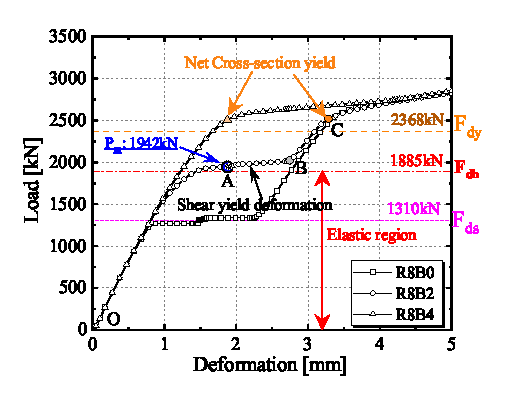
\includegraphics[width=\linewidth]{imgs/ch5/LD-A-R8Fdh.eps}
      \caption{R8 case}
      \label{fig-r8fdh}
    \end{subfigure}
\caption{The relationship between analysis result $P_{ss}$ and design bearing yield strength $F_{dh}$ of hybrid joint}
\label{fig-fdbpss}
\end{figure}

Tab.\ref{tab-assls} shows design strength and analyses results for each case in SLS, in which the bolt shear yield strength of the hybrid joint was calculated using Eq.\ref{eq-fdb}, as presented in this study. This equation predicts well for the case of hybrid joints where the bearing bolts do not fasten the preload (within an error of 2\% in the cases of R12B2-NCF and R12B4-NCF). Moreover, because this equation does not consider the preload of the bearing-type joint, the analysis value of the hybrid joint, in which the Interference fit bolt was fastened to the preload, was slightly higher than the calculated value. Except for R8B4, the errors were within 5\%. Because the preload of bolt No. 2 of the R8B4 case did not drop sharply or enter the shear yield state, this residual preload still resisted the tensile force as friction. Thus, the shear yield load obtained by the R8B4 case was slightly larger compared to the other cases.

\begin{table}[htbp]
\caption{Serviceability limit state design strength and analysis result of each case (Unit: kN)}
\label{tab-assls}
\centering
\scalebox{0.75}{
\begin{tabular}{@{}cccccccccc@{}}
\toprule
\begin{tabular}[c]{@{}c@{}}Case\\ Name\end{tabular} &
  \begin{tabular}[c]{@{}c@{}}Desgin\\ Slip Strength\\ $F_{ds}$\end{tabular} &
  \begin{tabular}[c]{@{}c@{}}Desgin NCS-Y \\ Strength\\ $F_{dy}$\end{tabular} &
  \begin{tabular}[c]{@{}c@{}}Design BS-Y \\Strength\\ $F_{db}$\end{tabular} &
  \begin{tabular}[c]{@{}c@{}}0.2 mm\\ Slip load\\ $P_{0.2s}$\end{tabular} &
  \begin{tabular}[c]{@{}c@{}}Bolt shear\\ Yield load\\ $P_{bsy}$\end{tabular} & 
  \begin{tabular}[c]{@{}c@{}}serviceability \\limit load\\$P_{ss}$ \end{tabular} &
  $\displaystyle{\frac{P_{0.2s}}{ F_{ds}}}$ &
  $\displaystyle{\frac{P_{db}}{F_{bsy}}}$ &
  SLS \\ \midrule
R12-O     & 1968 & \multirow{9}{*}{2368} & 5409 & 1578 & -    & 1578 & 0.8  & -    & Slip                \\
R12-B2    & 1968 &                       & 2542 & 1835 & 2603 & 2500 & 0.93 & 1.02 & NCS-Y \\
R12B2-NCF & 1968 &                       & 2542 & 1729 & 2500 & 2500 & 0.88 & 0.98 & NCS-Y \\
R12-B4    & 1968 &                       & 3115 & 1935 & 3206 & 2501 & 0.98 & 1.03 & NCS-Y \\
R12B4-NCF & 1968 &                       & 3115 & 1780 & 3130 & 2500 & 0.9  & 1.00 & NCS-Y \\
R10-B2    & 1640 &                       & 2213 & 1804 & 2242 & 2242 & 1.10 & 1.01 & BS-Y    \\
R10-B4    & 1640 &                       & 2787 & 1844 & 2873 & 2501 & 1.12 & 1.03 & NCS-Y \\
R8-B2     & 1312 &                       & 1886 & 1575 & 1942 & 1942 & 1.20 & 1.03 & BS-Y    \\
R8-B4     & 1312 &                       & 2459 & 1721 & 2608 & 2501 & 1.31 & 1.06 & NCS-Y \\ \bottomrule
\multicolumn{10}{r}{Where: NCS-Y:Net Cross-Section Yield; BS-Y: Bolt Shear Yield}
\end{tabular}}
\end{table}



\section{Conclusions}

To address issues of reduced slip load and interference in long bolted joints, this chapter proposed a hybrid joint combining Interference Fit Bolts (IFBs) and High-Strength Bolts (HSBs). Finite element analysis was conducted to evaluate the mechanical behavior of the hybrid joint.

\subsubsection*{Load transfer mechanisms}
\begin{itemize}
    \item The hybrid joint effectively increased strength and reduced joint length by using IFBs at both ends of slip-critical bolted joints. IFBs, unaffected by slip strength, provided higher bearing strength, ensuring adequate strength while shortening joint length.
    \item Using only one IFB at each end of long joints (over 8 rows) is not recommended due to potential local shear yield before net cross-sectional yield. At least two IFBs at each end are required to prevent excessive resistance on a single bolt.
\end{itemize}

\subsubsection*{Serviceability and design recommendations}
\begin{itemize}
    \item The bearing-critical strength of hybrid joints can be calculated using Eq.\ref{eq-fdb}, and net cross-sectional failure is recommended over bearing failure to maximize load-bearing capacity.
    \item Shortening a 12-row joint to an 8-row hybrid joint maintained slip strength while improving serviceability limit strength by 58\% (R8B2) and 23\% (R8B4) compared to 12-row friction joints. The reduction factor of slip strength can be ignored in shorter joints.
\end{itemize}


